% 导言区
\documentclass[UTF8]{article}%book ,report ,letter
\usepackage{geometry}%页边距设置
\geometry{a4paper,scale=0.85}
%\geometry{left=1.5cm,right=1.5cm,top=2.0cm,bottom=1.5cm}
\usepackage{diagbox}
\usepackage{ctexcap}%采用中文标题宏包(标题是中文的)
\usepackage{graphicx}%图片包
\usepackage{color}%彩色文本
\usepackage{amsmath}
\usepackage{caption2}
\usepackage{enumerate}
\usepackage{hyperref} %超链接包
\usepackage{amsmath}
\usepackage{hyperref} %超链接包
\usepackage{amsfonts }%阿拉伯字母
%覆盖超链接红框
\hypersetup{
	colorlinks=true,
	linkcolor=black
}
\usepackage{algorithm}
\usepackage[noend,compatible]{algpseudocode}
% Use the  Input / Output
\renewcommand{\algorithmicrequire}{ \textbf{INPUT:}} %Use Input in the format of Algorithm  
\renewcommand{\algorithmicensure}{ \textbf{OUTPUT:}} %UseOutput in the format of Algorithm  
\makeatletter\renewcommand{\ALG@name}{\textbf{Algorithm}} \makeatother
\title{\heiti 2019春招实习生面经}
\author{\kaishu LukeAlanLee}
\date{\today}

% 正文区(文稿区)
\begin{document}
	\maketitle %让头部内容在正文区显示
	\tableofcontents
	 \newpage
	\section{统计学习方法}
	泛化误差上界:至少以$1-\delta$的概率有$R(F)<=\hat{R}(f)+\epsilon(d,N,\delta)$
	\newpage
	\section{感知机}
	\begin{enumerate}
		\item 感知机是一种线性分类模型,属于判别模型
		\item 模型:寻找分离超平面;
		\item 损失函数:误分类样本到超平面的距离,误分类样本数不适用因为不连续;
		\item 学习算法:随机梯度下降
	\end{enumerate}
	\newpage
	\section{K近邻}
	三要素:
	\begin{enumerate}		
		\item[1.]k值的选择
		\item[2.] 距离度量
		\item[3.] 分类决策规则
	\end{enumerate}
	\subsection{kd树}
	kd树是一种二叉树,表示对k维空间的一个划分;
	通常,依次选择坐标轴对空间进行切分,选择训练实例点在选定坐标轴的中位数为切分点,这样得到的kd树是平衡的。(平衡的kd树的搜索效率未必是最高的)
	
	\newpage    
	\section{朴素贝叶斯}
	\begin{enumerate}
		\item 生成模型,学习联合概率分布
		\item 基本假设:用于分类的特征在类确定的条件下是条件独立的(特征向量$X$的每一维度对于输出的条件独立性)
		\item 后验概率最大化等价于期望风险最小化,推导:
		\begin{itemize}
			\item 假设采用0-1损失函数,朴素贝叶斯法的期望风险是对于联合分布$P(X,Y)$取的,因此相当于对于给定输出类别时的条件期望求和$$R_{exp}(f)=E_X\sum\limits_{k=1}^K[L(c_k,f(X))]P(c_k|X)$$
			\item 则对于给定的输入$x$,使其后验概率最大化的类别即为使期望风险最小化的输出。
		\end{itemize}
		\item 损失函数:误分类样本到超平面的距离,误分类样本数不适用因为不连续;
		\item 学习算法:随机梯度下降
		\item 贝叶斯估计
		
	\end{enumerate}
	
	\newpage
	\section{决策树}
	学习步骤:特征选择、决策树的生成、决策树的修剪
	\subsection{基本概念}
	\begin{enumerate}
		\item 熵(entropy):表示随机变量不确定性的度量$P(X=x_i)=p_i, i=1,2,...,n$,则其熵为:$$H(X)=-\sum\limits_{i=1}^n p_i\log p_i$$
		可以看出,熵的取值只与$X$的分布有关而与其取值无关,因此也可以记为:$$H(p)=-\sum\limits_{i=1}^n p_i\log p_i$$
		\item 条件熵:设有随机变量$(X,Y)$的联合概率分布为:$$P(X=x_i,Y=y_j)=p_{ij}, i=1,2,...,n, j=1,2,...,m$$
		在给定$X$的条件下$Y$的条件熵记为:$H(Y|X)$,定义为$X$给定条件下$Y$的条件概率分布的熵对$X$的数学期望:
		$$H(Y|X)=\sum\limits_{i=1}^n p_iH(Y|X=x_i)$$
		一般的,$$H(X,Y)=-\sum\limits_{x\in X} \sum\limits_{y \in Y } p(x,y)\log p(x,y)$$
		$$H(Y|X)=H(X,Y)-H(X) $$
		\item 信息增益:表示得知特征$X$的信息而使得类别$Y$的信息的不确定性较少的程度;一般地,
		$H(Y)-H(Y|X)$成为$(X,Y)$的互信息,	而特征$A$对训练数据集$D$的信息增益$g(D,A)$为:$$g(D,A)=H(D)-H(D|A)$$
		\item 信息增益比:特征$A$对训练数据集$D$的信息增益比$g_R(D,A)$定义为:
		$$g_R(D,A)=\frac{g(D,A)}{H_A(D)}$$
		$${H_A(D)}=-\sum_{i=1}^{n}\frac{|D_i|}{|D|}\log_2\frac{|D_i|}{|D|}$$
	\end{enumerate}
	
	\subsection{决策树的生成}
	\subsubsection{ID3算法}
	思想:从根节点,在每一个节点上选择当前信息增益最大的特征作为结点特征,由该特征的不同取值建立子节点,再对子节点递归运用上述算法,直到所有特征的信息增益很小或没有特征可以选择为止,得到一棵决策树。\\
	\emph{注意事项: }在子节点上进行的是特征对训练数据的子集计算信息增益。
	\subsubsection{C4.5算法}
	对ID3算法进行了改进,在生成过程中用信息增益比来选择特征。
	\subsection{决策树剪枝}
	决策树的损失函数定义为:
	$$C_\alpha(T)=C(T)+\alpha|T|
	=-\sum_{t=1}^{|T|}\sum_{k=1}^{K}N_{tk}\log\frac{N_{tk}}{N_t}$$
	$C(T)$表示模型对训练数据的预测误差,$|T|$表示模型的复杂度(树的深度),$\alpha\geq0$平衡二者之间的关系。
	\\进行剪枝时,将某一组的叶节点回缩至其父节点,若收缩后新的损失不大于旧的损失,则进行剪枝(收缩)。
	\subsection{CART算法}
	\subsubsection{最小二乘回归树}
	\newpage
	\subsubsection{CART决策树}
	利用基尼指数作为决策指标,对所有可能的特征及其所有可能的取值计算在对应处切分,计算基尼指数,选择基尼指数最小的切分点将训练集划分为两个子集,在子集上递归调用上述方法,直到满足停止条件。
	\subsubsection{CART剪枝}
	对整体树$T_0$中的每一个节点$t$,计算$$g(t)=\frac{C(t)-C(T_t)}{|T_t|-1}$$
	其中,$C(t)$是以$t$为单结点树的训练误差,$C(T_t)$是以$t$为根节点的子树$T_t$的训练误差,$|T_t|$是子树$T_t$的叶节点数。
	\\从$T_0$中减去$g(t)$最小的子树$T_t$,将得到的子树记为$T_1$,再从$T_1$减去$g(t)$最小的子树,如此循环下去直到决策树变为只剩根节点。
	\\最后采用交叉验证法从$T_0,T_1,...,T_n$中选出最优子树$T_\alpha$
	
	\newpage
	\section{线性回归}
		\subsection{线性回归的收缩与子集}
			\begin{enumerate}
				\item 为什么要进行收缩或选择子集
					\begin{itemize}
						\item 在线性回归上下文中,子集意味着从可用变量中选择要包含在模型中的子集,从而减少其维数。
						\item 收缩意味着减小系数估计的大小,如果系数缩小到恰好为零,则相应的变量将退出模型。因此,这种情况也可以看作是一种子集。
						\item \color{red}线性回归估计倾向于具有低偏差和高方差。\color{black}通过收缩与子集可以降低模型复杂性,倾向于减少方差,但代价是引入更多偏差。我们的目标是寻找一个偏差和方差之和最小的自己,从而改进模型。
						\item 增强模型的可解释性:过多的变量导致其相互之间的关系难以把握。
					\end{itemize}
				\item 简单的线性回归
				 $$
				 f(X)=\beta_{0}+\sum_{j=1}^{p} X_{j} \beta_{j}
				 $$
				 $p$为变量的个数。使用“普通最小二乘法”估计上述模型参数,以最小化残差平方和$\operatorname{RSS}(\beta)=\sum_{i=1}^{N}\left(y_{i}-f\left(x_{i}\right)\right)^{2}$为目标,易得上式具有解析解:
				 $$
				 \hat{\beta}=\left(\mathbf{X}^{T} \mathbf{X}\right)^{-1} \mathbf{X}^{T} \mathbf{y}
				 $$
				 \item 最佳子集回归
				 	\begin{itemize}
				 		\item 选择线性回归变量子集的直接方法是尝试所有可能的组合,并选择一个最小化损失的组合。
				 	\end{itemize}
			 	\item 岭回归
				 	\begin{itemize}
				 		\item 不直接选择变量,而是通过惩罚系数使其接近0以实现“选择”的目的,可以视为以连续方式降低模型复杂度。
				 		\item 岭回归的损失函数
				 		$$
				 		L_{ridge}(\hat{\beta})=\sum_{i=1}^{n}\left(y_{i}-x_{i} \hat{\beta}\right)^{2}+\lambda \sum_{j=1}^{m} \hat{\beta}_{j}^{2}=\|y-X \hat{\beta}\|^{2}+\lambda\|\hat{\beta}\|^{2}
				 		$$
				 		\item 最小化该损失函数得到:
				 		$$
				 		\hat{\beta}_{\text { ridge }}=\left(\mathbf{X}^{T} \mathbf{X}+\lambda \mathbf{I}\right)^{-1} \mathbf{X}^{T} \mathbf{y}
				 		$$
				 		\item 岭回归的偏差和方差公式:
				 		$$
				 		\begin{array}{c}{\operatorname{Bias}\left(\hat{\beta}_{\text {ridge}}\right)=-\lambda\left(X^{\prime} X+\lambda I\right)^{-1} \beta} \\ {\operatorname{Var}\left(\hat{\beta}_{\text {ridge}}\right)=\sigma^{2}\left(X^{\prime} X+\lambda I\right)^{-1} X^{\prime} X\left(X^{\prime} X+\lambda I\right)^{-1}}\end{array}
				 		$$
				 		\item 求解$\lambda$时使用交叉验证尝试不同的值,并选择一个最小化测试数据上交叉验证错误的值。
				 	\end{itemize}
		 		\item LASSO 
		 			\begin{itemize}
		 				\item 本质上与岭回归非常相似, 但使用的惩罚项为L1
		 				\item L1 与 L2 的区别决定了岭回归更适用于大多数变量对预测有影响时;而Lasso适用于少数变量真正对预测有影响(即多重共线性问题的解决方式不同)。
		 				\item Lasso的损失函数:
		 				$$
		 				L_{lasso}(\hat{\beta})=\sum_{i=1}^{n}\left(y_{i}-x_{i}^{\prime} \hat{\beta}\right)^{2}+\lambda \sum_{j=1}^{m}\left|\hat{\beta}_{j}\right|
		 				$$
		 				\item L1不可微,故只能用数值方法求解
		 				\item LASSO的变量选择过于依赖数据,因而不稳定
		 			\end{itemize}
	 			\item 弹性网:将岭回归和LASSO的惩罚结合起来,以获得两全其美的效果。
	 			\begin{description}
	 				\item 损失函数:$$
	 				L_{\text {exet}}(\hat{\beta})=\frac{\sum_{i-1}^{n}\left(y_{i}-x_{i}\hat{\beta}\right)^{2}}{2 n}+\lambda\left(\frac{1-\alpha}{2} \sum_{j=1}^{m} \hat{\beta}_{j}^{2}+\alpha \sum_{j=1}^{m}\left|\hat{\beta}_{j}\right|\right)
	 				$$
	 			\end{description}
	 			\item 最小角度回归(LAR)
	 				\begin{itemize}
	 					\item 
	 				\end{itemize}
 				\item 主成分回归
 				\begin{itemize}
 					\item 利用PCA做特征重构,再将重构出的特征用于简单线性回归
 				\end{itemize}
 			\item 偏最小二乘法(PLS)
 			\begin{itemize}
 				\item 尽管PLS根据需要缩小了Z(重构特征)中的低方差分量,但它有时会使高方差分量膨胀,这可能导致在某些情况下更高的预测误差。
 			\end{itemize}
			\end{enumerate}
		
	
	\newpage
	\section{逻辑斯蒂回归与最大熵模型}
	\subsection{逻辑斯蒂回归模型}
	对于二项LR模型,它的形式是
	$$P(Y=1|x)=\frac{\exp(w \cdot x+b)}{1+\exp(w \cdot x+b)}$$
	$$P(Y=0|x)=\frac{1}{1+\exp(w \cdot x+b)}$$
	把两个式子统一得到似然函数,然后取对数,对于对数似然函数求极大值得到w的估计值即可。
	对于过拟合问题可以采用L1正则化或者L2正则化。
	\subsection{最大熵模型}
	最大熵模型通俗点讲可以理解在满足约束条件的模型中选取熵最大的,对于给定的输入模型的输出是条件概率$P(Y|X)$;\\
	对条件熵的最大化过程可以转化为其负值得最小化,然后引入拉格朗日乘子将约束优化问题转化为它的无约束优化问题,
	然后再对它的对偶问题进行求解,将极小极大问题转化为极大极小问题,先求出最优的满足约束条件的最大熵模型,再对模型进行参数优化。
	\newpage
	\section{支持向量机}
	间隔最大化的直观解释:对训练数据以充分大的确信度进行分类。\\
	SMO:序列最小化(sequential minimal optimization)
	
	\newpage    
	\section{EM算法及其推广}
	\textcolor{red}{最简单的了解EM算法思路的是K-Means算法:}
	\\在K-Means聚类时,每个聚类簇的质心是隐含数据。我们会假设K个初始化质心,即EM算法的E步;然后计算得到每个样本最近的质心,并把样本聚类到最近的这个质心,即EM算法的M步。重复这个E步和M步,直到质心不再变化为止,这样就完成了K-Means聚类。
	\\EM算法流程:
	\\对于观察数据$x=(x^{(1)},x^{(2)},...,x^{(m)})$,联合分布$p(x,z;\theta)$,条件分布$p(z|x;\theta)$,最大迭代次数$J$.
	\\1) 随机初始化模型参数$\theta$的初值$\theta^0$;
	\\2)从$j=1$到$J$迭代:
	\\2.a)E步:计算联合分布的条件概率期望:$$Q_i(z^{(i)}) = P( z^{(i)}|x^{(i)},\theta^{j}))$$
	$$L(\theta, \theta^{j}) = \sum\limits_{i=1}^m\sum\limits_{z^{(i)}}Q_i(z^{(i)})log{P(x^{(i)}, z^{(i)};\theta)}$$
	2.b) M步:极大化$L(\theta, \theta^{j})$,得到$ \theta^{j+1}$:
	$$\theta^{j+1} = arg \max \limits_{\theta}L(\theta, \theta^{j})$$
	2.c) 如果$ \theta^{j+1}$已收敛,则算法结束。否则继续回到步骤2.a)进行E步迭代。
	\\	\textcolor{red}{1.实际上},在E步,我们所做的事情是固定模型参数的值,优化隐含数据的分布,而在M步,我们所做的事情是固定隐含数据分布,优化模型参数的值。
	\textcolor{red}{2.EM算法是初值敏感的;}
	
	\newpage
	\section{隐马尔科夫模型}
	
	三个经典的问题:
	\begin{enumerate}		
		\item[1.]评估观察序列概率
		\item[2.]模型参数学习问题
		\item[3.]预测问题
	\end{enumerate}
	
	\subsection{评估观察序列概率}
	
	\subsubsection{前向算法}
	给定隐马尔科夫模型$\lambda = (A,B,\pi)$,观测序列$O=(o_1,o_2,...o_T)$;
	定义时刻t时隐藏状态为$q_i$, 观测状态的序列为$o_1,o_2,...,o_t$的概率为前向概率,记为:
	$$\alpha_t(i) = P(o_1,o_2,...o_t, i_t =q_i | \lambda)$$
	\\使用前向算法求解观测序列概率$P(O|\lambda)$
	\\1.初始化时刻1的各个隐藏状态前向概率:$$\alpha_1(i) = \pi_ib_i(o_1),\; i=1,2,...N$$
	2.递推时刻2,3,...,T时刻的前向概率:$$\alpha_{t+1}(i) = \Big[\sum\limits_{j=1}^N\alpha_t(j)a_{ji}\Big]b_i(o_{t+1}),\; i=1,2,...N$$
	3.计算最终结果:$$P(O|\lambda) = \sum\limits_{i=1}^N\alpha_T(i)$$
	
	\subsubsection{后向算法}
	定义时刻t时隐藏状态为$q_i$,从时刻$t+1$到最后时刻$T$的观测状态的序列为$o_{t+1},o_{t+2},...o_T$的概率为后向概率记为:$$\beta_t(i) = P(o_{t+1},o_{t+2},...o_T| i_t =q_i , \lambda)$$
	给定隐马尔科夫模型$\lambda = (A,B,\pi)$,观测序列$O=(o_1,o_2,...o_T)$;
	\\使用前向算法求解观测序列概率$P(O|\lambda)$
	\\1.初始化时刻1的各个隐藏状态后向概率:$$\beta_T(i) = 1,\; i=1,2,...N$$
	2.递推时$T-1,T-2,...1$时刻的后向概率:$$\beta_{t}(i) = \sum\limits_{j=1}^{N}a_{ij}b_j(o_{t+1})\beta_{t+1}(j),\; i=1,2,...N$$
	3.计算最终结果:$$P(O|\lambda) = \sum\limits_{i=1}^N\pi_ib_i(o_1)\beta_1(i)$$
	
	\subsubsection{常用概率计算}
	1.给定模型$\lambda$和观测序列$O$,在时刻$t$处于状态$q_i$的概率记为:
	$$\gamma_t(i) = P(i_t = q_i | O,\lambda) = \frac{P(i_t = q_i ,O|\lambda)}{P(O|\lambda)}$$
	利用前向概率和后向概率的定义可知:$$P(i_t = q_i ,O|\lambda) = \alpha_t(i)\beta_t(i)$$
	所以:$$\gamma_t(i) = \frac{ \alpha_t(i)\beta_t(i)}{\sum\limits_{j=1}^N \alpha_t(j)\beta_t(j)}$$
	
	2.给定模型$\lambda$和观测序列$O$,在时刻$t$处于状态$q_i$,且在时刻$t+1$处于状态$q_{i+1}$的概率记为:$$\xi_t(i,j) = P(i_t = q_i, i_{t+1}=q_j | O,\lambda) = \frac{ P(i_t = q_i, i_{t+1}=q_j , O|\lambda)}{P(O|\lambda)}$$
	由前向后向概率来表示为:$$P(i_t = q_i, i_{t+1}=q_j , O|\lambda) = \alpha_t(i)a_{ij}b_j(o_{t+1})\beta_{t+1}(j)$$
	则有:$$\xi_t(i,j) = \frac{\alpha_t(i)a_{ij}b_j(o_{t+1})\beta_{t+1}(j)}{\sum\limits_{r=1}^N\sum\limits_{s=1}^N\alpha_t(r)a_{rs}b_s(o_{t+1})\beta_{t+1}(s)}$$
	3.对状态求和可得到其他一些有用的概率
	\\在观测序列O下状态i出现的期望值:$\sum\limits_{t=1}^T\gamma_t(i)$
	\\在观测序列O下由状态i转移的期望值:$\sum\limits_{t=1}^{T-1}\gamma_t(i)$
	\\在观测序列O下由状态i转移到状态j的期望值:$\sum\limits_{t=1}^{T-1}\xi_t(i,j)$
	
	\subsection{模型的参数估计}
	\subsubsection{给定状态序列和观测序列}
	使用极大似然估计可得,
	\\状态转移矩阵:$$A = \Big[a_{ij}\Big], \;where\; a_{ij} = \frac{A_{ij}}{\sum\limits_{s=1}^{N}A_{is}}$$
	观测状态概率矩阵为:$$B= \Big[b_{j}(k)\Big], \;{where}\; b_{j}(k) = \frac{B_{jk}}{\sum\limits_{s=1}^{M}B_{js}}$$
	假设所有样本中初始隐藏状态为$q_i$的频率计数为$C(i)$,那么初始概率分布为:
	$$\Pi = \pi(i) = \frac{C(i)}{\sum\limits_{s=1}^{N}C(s)}$$
	\newpage
	\subsubsection{鲍姆-韦尔奇(Baum-Welch)算法(也就是EM算法)}
	假设之给定了$D$个长度为$T$的观测序列$\{(O_1), (O_2), ...(O_D)\}$,而没有给出对应的状态序列,目标是学习隐马尔科夫模型的参数,
	求解的流程如下:
	1.随机初始化所有的$\pi_i, a_{ij},b_{j}(k)$ \\
	2. 对于每个样本$d = 1,2,...D$,用前向后向算法计算$\gamma_t^{(d)}(i),\xi_t^{(d)}(i,j), t =1,2...T$\\
	3.更新模型参数:
	$$\pi_i =  \frac{\sum\limits_{d=1}^D\gamma_1^{(d)}(i)}{D}$$
	$$a_{ij} = \frac{\sum\limits_{d=1}^D\sum\limits_{t=1}^{T-1}\xi_t^{(d)}(i,j)}{\sum\limits_{d=1}^D\sum\limits_{t=1}^{T-1}\gamma_t^{(d)}(i)}$$
	$$b_{j}(k) = \frac{\sum\limits_{d=1}^D\sum\limits_{t=1, o_t^{(d)}=v_k}^{T}\gamma_t^{(d)}(j)}{\sum\limits_{d=1}^D\sum\limits_{t=1}^{T}\gamma_t^{(d)}(j)}$$
	4. 如果$\pi_i, a_{ij},b_{j}(k)$的值已经收敛,则算法结束,否则回到第2步继续迭代。
	
	\subsection{隐藏状态序列预测问题}
	即给定模型和观测序列,求给定观测序列条件下,最可能出现的对应的隐藏状态序列。\\
	\emph{\large 维特比算法:}\\
	两个局部状态:\\
	1.时刻t隐藏状态为i所有可能的状态转移路径$i_1,i_2,...i_t$中的概率最大值:
	$$\delta_t(i) = \max_{i_1,i_2,...i_{t-1}}\;P(i_t=i, i_1,i_2,...i_{t-1},o_t,o_{t-1},...o_1|\lambda),\; i =1,2,...N$$
	由$\delta_t(i)$的定义可以得到$\delta$的递推表达式:
	\begin{align} 
	\delta_{t+1}(i)
	& =  \max_{i_1,i_2,...i_{t}} \; P(i_{t+1}=i,i_1,i_2,...i_{t},o_{t+1},o_{t},...o_1|\lambda)\\ 
	& = \max_{1 \leq j \leq N}\;[\delta_t(j)a_{ji}]b_i(o_{t+1})
	\end{align}
	2.时刻t隐藏状态为i所有单个状态转移路径$(i_1,i_2,...i_{t-1},i)$中概率最大的转移路径中第t−1个节点的隐藏状态为$\phi_t(i)$,由1.可得其递推表达式为:
	$$\Psi_t(i) = arg \; \max_{1 \leq j \leq N}\;[\delta_{t-1}(j)a_{ji}]$$
	维比特算法流程:\\
	输入:隐马尔科夫模型$\lambda = (A,B,\pi)$,观测序列$O=(o_1,o_2,...o_T)$;
	输出:最有可能的隐藏状态序列$I^*= \{i_1^*,i_2^*,...i_T^*\}$\\
	1.初始化局部状态:
	$$\delta_1(i) = \pi_ib_i(o_1),\;i=1,2...N$$
	$$\Psi_1(i)=0,\;i=1,2...N$$
	2.进行动态规划递推时刻t=2,3,...,T时刻的局部状态:
	$$\delta_{t}(i) = \max_{1 \leq j \leq N}\;[\delta_{t-1}(j)a_{ji}]b_i(0_{t}),\;i=1,2...N$$
	$$\Psi_t(i) = arg \; \max_{1 \leq j \leq N}\;[\delta_{t-1}(j)a_{ji}],\;i=1,2...N$$
	3.算时刻T最大的$\Psi_T(i)$,即为最可能隐藏状态序列出现的概率。计算时刻T最大$\Psi_t(i)$,即为时刻T最可能的隐藏状态:
	$$P* = \max_{1 \leq j \leq N}\delta_{T}(i)$$
	$$i_T^* = arg \; \max_{1 \leq j \leq N}\;[\delta_{T}(i)]$$
	4.利用局部状态$\Psi(i) $开始回溯。对于$t=T-1,T-2,...,1$
	$$i_t^* = \Psi_{t+1}(i_{t+1}^*)$$
	最终得到最有可能的隐藏状态序列$I^*= \{i_1^*,i_2^*,...i_T^*\}$\\
	\textcolor{red}{维特比算法的核心是定义动态规划的局部状态与局部递推公式.}
	
	\newpage
	\section{条件随机场}
	\subsection{什么样的问题需要CRF模型}
	\subsection{条件随机场}
	随机场:随机场是由若干个位置组成的整体,当给每一个位置中按照某种分布随机赋予一个值之后,其全体就叫做随机场。
	
	马尔科夫随机场:假设随机场中某一个位置的赋值仅仅与和它相邻的位置的赋值有关,和与其不相邻的位置的赋值无关,则称其为马尔科夫随机场。
	
	条件随机场(Conditional Random Fields,简称 CRF):设$X$与$Y$是随机变量,$P(Y|X)$是给定$X$时$Y$的条件概率分布,若随机变量$Y$构成的是一个马尔科夫随机场,则称条件概率分布$P(Y|X)$是条件随机场。
	
	线性链条件随机场:$X$与$Y$有相同的结构的CRF就构成了线性链条件随机场(Linear chain Conditional Random Fields,简称 linear-CRF)。\\
	数学定义:设$X =(X_1,X_2,...X_n),\;\;Y=(Y_1,Y_2,...Y_n)$均为线性链表示的随机变量序列,在给定随机变量序列$X$的情况下,随机变量$Y$的条件概率分布$ P(Y|X) $构成条件随机场,即满足马尔科夫性:
	$$P(Y_i|X,Y_1,Y_2,...Y_n) = P(Y_i|X,Y_{i-1},Y_{i+1})$$
	则称$ P(Y|X) $为线性链条随机
	\subsubsection{线性链条件随机场的参数化形式}
	定义在$Y$节点上的状态特征:
	$$s_l(y_i, x,i),\;\; l =1,2,...L$$
	$L$是定义在该节点的特征函数的总个数,$i$是当前节点在序列的位置。
	定义在Y上下文的局部特征函数,这类特征函数只和当前节点和上一个节点有关,称为转移特征,记为:
	$$t_k(y_{i-1},y_i, x,i),\;\; k =1,2,...K$$
	$K$是定义在该节点的局部特征函数的总个数,$t_k,s_l\in\{0,1\}$,表示满足特征条件或者不满足特征条件。同时,可以为每个特征函数赋予一个权值,用以表达 对这个特征函数的信任度。\\
	假设$t_k$的权重系数是$\lambda_k$,$s_l$的权重系数是$\mu_l$,则linear-CRF由我们所有的$t_k,\lambda_k,s_l,\mu_l$共同决定.\\
	则linear-CRF的参数化形式如下:
	$$P(y|x) = \frac{1}{Z(x)}exp\Big(\sum\limits_{i,k} \lambda_kt_k(y_{i-1},y_i, x,i) +\sum\limits_{i,l}\mu_ls_l(y_i, x,i)\Big)$$
	其中,$Z(x)$为规范化因子:
	$$ Z(x) =\sum\limits_{y} \exp\Big(\sum\limits_{i,k} \lambda_kt_k(y_{i-1},y_i, x,i) +\sum\limits_{i,l}\mu_ls_l(y_i, x,i)\Big)$$
	回到特征函数本身,每个特征函数定义了一个linear-CRF的规则,则其系数定义了这个规则的可信度。所有的规则和其可信度一起构成了我们的linear-CRF的最终的条件概率分布。
	\\记:\\
	$$f_k(y_{i-1},y_i, x,i)= \begin{cases} t_k(y_{i-1},y_i, x,i) & {k=1,2,...K_1}\\ s_l(y_i, x,i)& {k=K_1+l,\; l=1,2...,K_2} \end{cases}$$
	$$w_k= \begin{cases} \lambda_k & {k=1,2,...K_1}\\ \mu_l & {k=K_1+l,\; l=1,2...,K_2} \end{cases}$$
	得到简化的linear-CRF参数化表示:
	$$P(y|x) =  \frac{1}{Z(x)}exp\sum\limits_{k=1}^Kw_kf_k(y,x)$$
	$$Z(x) =\sum\limits_{y}exp\sum\limits_{k=1}^Kw_kf_k(y,x)$$
	矩阵表示形式:
	$$M_i(x) = \Big[ M_i(y_{i-1},y_i |x)\Big] =  \Big[  exp(W_i(y_{i-1},y_i |x))\Big] = \Big[  exp(\sum\limits_{k=1}^Kw_kf_k(y_{i-1},y_i, x,i))\Big]$$
	我们引入起点和终点标记$y_0 =start, y_{n+1} = stop$, 这样,标记序列y的非规范化概率可以通过n+1个矩阵元素的乘积得到:
	$$P_w(y|x) =  \frac{1}{Z_w(x)}\prod_{i=1}^{n+1}M_i(y_{i-1},y_i |x)$$
	$$Z_w(x)=(M_1(x)M_2(x)...M_{n+1}(x)))_{start,stop}$$
	\newpage
	\flushleft
	模型的三个基本问题:
	\begin{enumerate}		
		\item[1.]评估观察序列概率
		\item[2.]模型参数学习问题
		\item[3.]预测问题
	\end{enumerate}
	\subsection{概率计算}
	用$\alpha_i(y_i|x)$表示序列位置$i$的标记是$y_i$,在起点处,定义:
	$$\alpha_0(y_0|x)= \begin{cases} 1 & {y_0 =start}\\ 0 & {else} \end{cases}$$
	则在位置$i+1$之前的部分标记序列的非规范化概率$\alpha_{i+1}(yi+1|x)$的递推公式:
	$$\alpha_{i+1}(y_{i+1}|x) = \alpha_i(y_i|x)M_{i+1}(y_{i+1},y_i|x) \;\; i=1,2,...,n+1$$
	\newpage
	\section{面经}
	\date{2019年3月8日} 
	\subsection{腾讯 TEG NLP组}
	一面:凉凉\\
	编程:\\
	1.使用二分查找在一个有序数组中查找某个数第一次出现的位置,如果没有找到返回插入的位置\\
	2.计算数组中和最大的子数组,返回最大和\\
	问简历:\\
	1.之前的实习都做了哪些工作;\\
	2.图像分类的项目:\\
	2.1用SVM如何实现的多分类,surft特征和sift特征的区别\\
	2.2迁移学习怎么做的?训练数据有多少,如何划分的?\\
	3.法律文本分类怎么做的,输入多少文本,每个文本的长度(n),用词向量look\_up的话得到的不就是$ n*m $了吗(总之要把整个系统从输入到输出都说明白)\\
	机器学习基础:\\
	1.讲一讲LR\\
	2.SVM的最优化目标为什么是$\frac{1}{2}||\omega||^2$(原因,而非推导)\\
	3.LR和SVM的正则化有什么区别?\\
	算法实现
	1.TensorFlow的lstm有哪些cell(单元)\\
	
	\date{2019年3月29日}
	\subsection{腾讯云}
	一面:通过\\
	仍旧是问简历\\
	1.LDA的原理\\
	2.讲一下HMM\\
	3.Attention 是怎么来的?\\
	4.双向RNN与单向RNN有什么不同\\
	5.word2vec的原理,transformer知道吗,bert知道吗?\\
	6.tf-idf特征怎么来的\\
	编程:\\
	1.Linux,普通用户,使用1001端口,无法调用,可能的原因; 普通用户能够使用的端口范围\\
	2.TensorFlow用的GPU还是CPU\\
	3.翻转一个整数n,比如12345,输出就是54321。\\
	(可能遇到的问题,1.负数,2.会越界溢出吗,int的范围$-2^{31} ---\;2^{31}-1$)\\
	4.一百个灯泡,从灭的状态开始,按一下打开,再按灭,再按再打开。第一遍按能被1整除的位置上的灯,第二遍按能被2整除的,依次类推直到按一遍能被100整除的,结束之后有哪些等是亮的?答案是平方数(1,4,9,16...)的灯是亮的,因为只有平方数的灯被按了奇数次,其他的都被按了偶数次。\\
	5.(因为简历上写了爬虫)爬虫是怎么做的,不会被ban吗\\
	二面:凉凉\\
	1.哪些情况下需要softmax,哪些不需要\\
	2.CNN 和 RNN 分别适用于哪些场景,比如适用哪些类型的数据(比如从频域和时域来讲),从非NLP领域举些例子\\
	3.做过哪些数据清洗\\
	4.什么样的数据容易导致过拟合,如何处理\\
	5.数学基础怎么样(回答简单推导了一下SVM)\\
	(回答都是已NLP方面举例,面试官说应该多接触一些其他领域)\\
	
	\date{2019年3月27日}
	\subsection{华为---算法工程师}
	一面:通过\\
	1.简历上的项目\\
	2.爬虫(聊了挺多)\\
	3.CNN是如何提取文本特征的,提取到的特征是什么类型的(特点)\\
	4.简单讲一下CNN的结构\\
	二面:通过\\
	1.如何使用HMM做NER\\
	2.attention机制,self-attention知道吗, Bert了解吗?\\
	3.使用python用一行找出句子中的所有回文词\\
	4.有读博的打算吗\\
	5.为什么选择华为\\
	
	\date{2019年4月1日}
	\subsection{百度深圳---NLP---现场面}
	1.实习项目;\\
	2.研究方向怎么做的,有自己提出的想法吗?\\
	3.C++实现一个字符串翻转,空间复杂度尽量低(传指针比较)。\\
	4.TensorFlow实现一个LSTM,给出Loss\\
	5.batch size个sequence len的文本, batch个label, TensorFlow实现一个二分类\\
	解决方法:假设可以用词向量,对每一个sequence len词做look\_up,得到的是[batch,seq.len,V]的三维矩阵,做reduce\_mean(可以解决seq len长度不同,因为都只剩1了)得到一个[batch,hidden]的隐藏层向量,然后在做$y=\omega x + b$得到batch size的输出,对输出做sigmoid,然后用交叉熵$y\log(\hat{y})+(1-y)\log{(1-\hat{y})}$返回损失。\\
	6.讲一下LDA的基本原理\\
	7.如何把不等长的句子转化成等长的向量:\\
	Encoder、Bow、CNN、 Bert\\
	8.100亿条已排序好的文本\\
	\center 
	a $\;$ 3\\
	b $\;$ 2\\
	b $\;$ 4\\
	c $\;$ 1\\
	c $\;$ 1\\
	...\\
	输出得到\\
	a $\;$  3\\
	b $\;$ 6\\
	c $\;$ 2\\
	...\\
	\flushleft
	\date{2019年4月17日}
	\subsection{今日头条 算法工程师}
		\begin{enumerate}
			\item 编程题,求逆序对(无重复、有重复)
			\item LSTM的结构
			\item sigmoid 和tanh的区别:在LSTM中,三个sigmoid门是决定信息是否继续走下去的,而tanh是将信息整理到区间(-1,1)的,也就是生成候选信息。
			\item 从LSTM扩展-GRU:
			\item GBDT 的T步是怎么做的?
			\item 了解哪些优化算法
			\item SVM的核函数怎么使用?
			\item batch normalization的作用,网络参数初始化方法;
			\begin{itemize}
				\item 在恰当的地方做了标准化(Normalization),在矩阵乘之后,在激活之前;
			\end{itemize}
		\end{enumerate}
	
		%LSTM结构
		\begin{figure}[H]
		\centering
		\noindent\makebox[\textwidth][c] {
			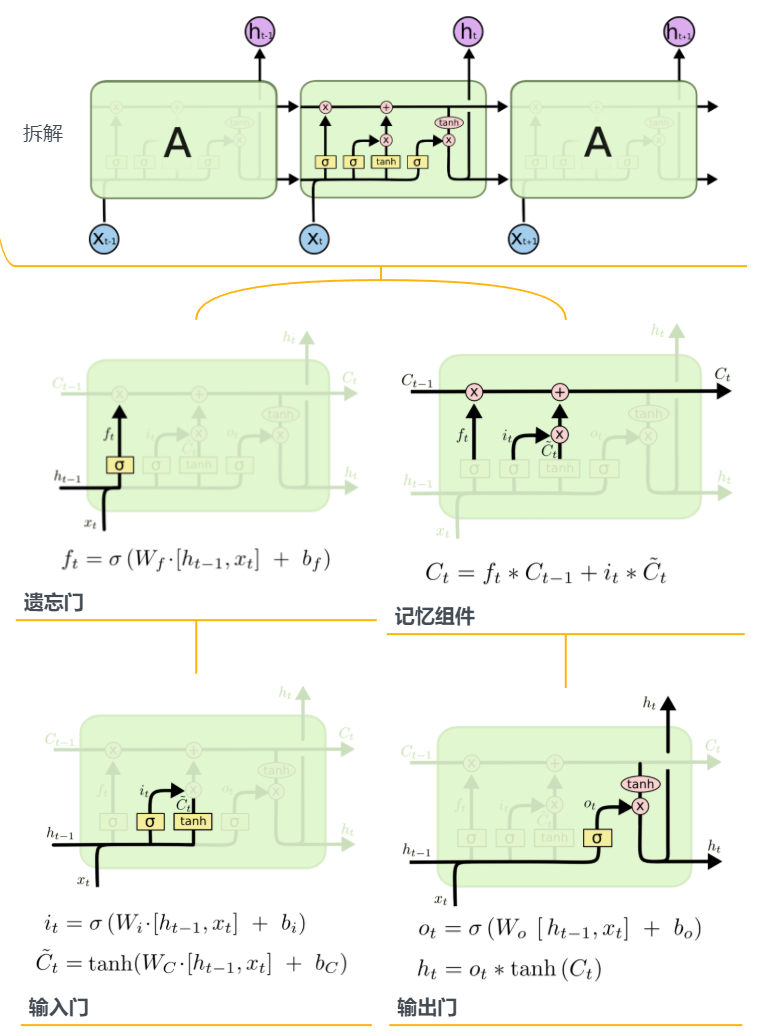
\includegraphics[width=0.7\paperwidth]{figures/LSTMAllInOne.png}}
		\caption{LSTMAllInOne}  %图片的名称
		\label{LSTMAllInOne}   %标签,用作引用
		\end{figure}
		\clearpage
		
		%GRU结构
		\begin{figure}[H]
		\centering
		\noindent\makebox[\textwidth][c] {
			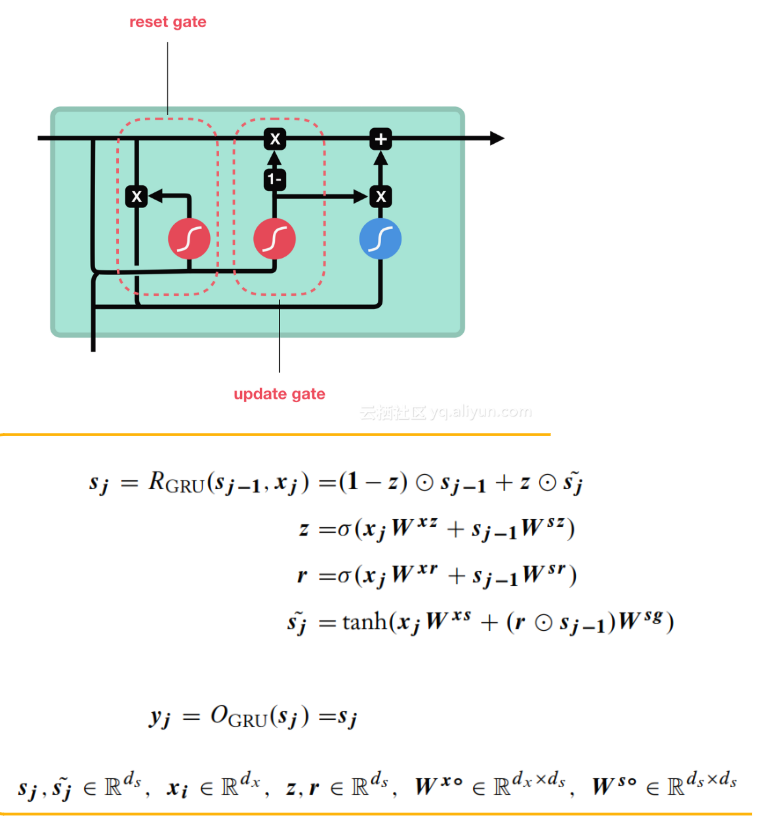
\includegraphics[width=0.5\paperwidth]{figures/GRU.png}}
		\caption{GRU}  %图片的名称
		\label{GRU}   %标签,用作引用
		\end{figure}
		\clearpage

	\subsection{一些可能会问到的问题}
	\par
	\begin{enumerate}
		
		\item 为什么ReLu要好过于tanh和sigmoid function?
			\begin{itemize}
				\item 首先,sigmoid函数将数值挤压到[0,1],存在两大不足:
					\begin{description}
						\item[a.] 函数饱和使梯度消失。当神经元的激活在接近0或1处时会饱和,梯度几乎为0,导致梯度消失,几乎就有没有信号通过神经传回上一层。
						\item[b.] 输出不是零中心的。如果输入神经元的数据总是正数,那么关于w的梯度在反向传播的过程中,将会要么全部是正数,要么全部是负数,这将会导致梯度下降权重更新时出现z字型的下降				
					\end{description}
				\item tanh函数将数值挤压到[-1,1],解决了sigmoid不是以零为中心的问题,但仍然存在饱和问题。
				\item ReLu具有单侧抑制(提供了网络的稀疏表达能力)、相对宽阔的兴奋边界、稀疏激活性等特性 
				\item Relu在激活区域是线性的,极大的提升了收敛效率,也无指数运算,减少了计算量。
			\end{itemize}
		\item ReLu的局限性
			\begin{itemize}
				\item 训练过程会导致神经元死亡
				\item 解决方法:Leaky ReLu
				\begin{equation} 
				f(x)=\begin{cases} 
				z   & z>0; \\ 
				az & z<=0.
				\end{cases} 
				\end{equation} \label{3}
			\end{itemize}
		\item 正则化为什么能够防止过拟合?
			\begin{description}
				\item \qquad 正则化可以防过拟合的原因是,数学上可以证明,加了正则项之后的估计出来的参数向量的长度严格小于不加的估计的向量长度。整体来看,有些分量的长度严格变小了,极端来看,可能某些分量被压缩至零。所以防止过拟合的最本质最根本原因就是估计出来的参数模长变小了;为什么模长会变小的数学证明,用到了矩阵范数和向量范数相容的一些性质。
				\item \qquad 变量选择或者特征选择,重点在选择,L2一般没有选择能力,L1才有选择能力;\color{red}而L1具有选择能力的本质,在于其满足符号相合性,即它有大概率将真实值为零参数估计为零,将真实值非零的参数估计为非零且保号。\color{black}所以两者结合来看,向量长度在变小,并且每个分量与真实值的符号大概率一致,当然最终结果就是该是零的分量压缩到零,实现变量选择,且实现了防止过拟合。
			\end{description} 
		\item 1.L1正则化和L2正则化的区别:
			\begin{itemize}
				\item 	L1正则化衡量的是曼哈顿距离,在使用的过程中会导致模型稀疏稀疏
				\item 	L2正则化衡量的是欧式距离,具有适用于任何维度数据的特点。
			\end{itemize}
		\item L1用于逻辑回归,C 是正则化参数,C 值从 0 增加至非常大会有什么变化?
		\item MLE的解是否总是存在,若存在是否唯一?
			\begin{itemize}
				\item 	MLE (最大似然估计)可能并不存在,如果 MLE 存在,那么它的解可能不是唯一的
				\item 解释:
					\begin{description}
						\item[1.] 如果似然函数的一阶导不存在,那么MLE就不存
						\item[2.] 似然函数取得极大值时对应的参数也不唯一,需要似然函数满足凸函数才唯一
					\end{description}
			\end{itemize}
		\item 词向量训练中使用负采样训练时的辅助变量是否可以用作词向量? 
		\item 辅助变量是否可以被替换成词向量来训练?
		\item 使用NCE loss训练词向量和使用hierarchical softmax训练有什么本质的不同?
		\item 树模型如ID3,C4.5的损失函数是什么? 和XGBoost有什么区别?
		\item 核方法除了在SVM中使用,还有哪些使用的场景?
		\item 使用Relu激活函数的多层感知机会出现什么样的问题?应该怎么解决?
		\item 如果一个方法上线以后发现和线下测试得到的结果不一样(线上效果较线下效果差劲),可能是哪里出了问题,应该怎么解决?
		\end{enumerate}
		\subsection{数学概念}
			\begin{enumerate}
			\color{red}
			\item VC-Dimension
				\color{black}
				\begin{itemize}
					\item shatter(”打散“):对于大小为${N}$的样本集合$\mathcal{D}$,如果 Hypothesis Set 可以做出所有$2^N$可能的种 dichotomy,则称这个样本能被 Hypothesis Set shatter,或者$\mathcal{H}$ shatter 了这${N}$个样本。
					\item Break Point 是第一个无法被 Hypothesis Set 所 shatter 的“点” 。
					\color{red}\item VC Dimension 是最后一个可以被 Hypothesis Set 所 shatter 的“点”。\color{black}
					\item 跟成长函数一样,Break Point 和 VC Dimension 也都属于 Hypothesis Set 本身的性质。不同的 Hypothesis Set 有其各自的 Break Point 和 VC Dimension 。
				\end{itemize}
			\item VC Dimension的性质
				\begin{description}
					\item[a.] 只要某个 Hypothesis Set 存在 VC Dimension,就一定有$E_{predict}(g)=E_{train}(g)$ is Probably Approximately Correct (PAC).也就是说由训练数据学得的模型,"真的 (PAC)" 能在未来的预测中表现的一样好。
					\item[b.] VC Dimension 越大,样本复杂度 (sample complexity) 就越高!
					\item 由公式\begin{equation}
					P\left( | E_{\text {predict}}(g)-E_{\text {train}}(g) | \geq \epsilon\right) \leq 2 \cdot \frac{2 \cdot \sum\limits_{i=0}^{k-1} \left( \begin{array}{c}{2 N} \\ {i}\end{array}\right)}{e^{2 \cdot \frac{1}{16} \cdot N \epsilon^{2}}}
					\end{equation}\label{4}
					其中的$k-1$即为 VC Dimension,由公式可知, VC Dimension越大,预测准确率与训练准确率差值超过一定范围的概率就越大,因此如果想要维持“越界概率”不变,就要进一步增大样本数$N$。
					\item[c.] \color{red} VC Dimension 越大,模型的”表达“能力就越强。\color{black}VC Dimension 是最后一个可以被 shatter 的“点”,也就是在样本数小于等于 VC Dimension 时, Hypothesis Set 可以“表达”所有可能的样本输出情况。这就是说 VC Dimension 越大,就意味着 Hypothesis Set 的”表达“能力就越强。
					\item[d.]  VC Dimension 是预测准确率优化中的矛盾点。
					\item 由(2)和(3)可知,VC Dimension表现出了模型的复杂度与“表达”能力之间的矛盾。增大VC Dimension能够提升模型的“表达”能力,但又会造成“越界概率”增大,模型复杂度提高。在实际中,样本量N的获取往往受到限制,不可能无限的提升,此时我们更关心的是在样本量有限时得到较高的预测准确率$E_{\text {predict}}(g)$,其中$g$表示假设空间中的某个假设。具体的,在样本量N足够大时,模型可以\color{red}$1-\delta$的概率\color{black}保证预测准确率:
					\begin{equation}
					E_{train} - \sqrt{\frac{16}{2 \cdot N} \cdot \ln \left(\frac{2 \cdot 2 \cdot \sum\limits_{i=0}^{k-1}(2 N)}{\delta}\right)} \leq \quad E_{\text {predict}}(g) \quad \leq { {E_{train}}(g)+\sqrt{\frac{16}{2 \cdot N} \cdot \ln \left(\frac{2 \cdot 2 \cdot \sum\limits_{i=0}^{k-1}(2 N)}{\delta}\right)}}
					\end{equation}\label{5}
					\item \quad 上述区间的由来:由公式(4),当训练样本$N$足够大时,预测准确率以大于等于$\epsilon$的误差偏离训练准确率的概率可以是一个足够小的值($2 \cdot \frac{2 \cdot \sum\limits_{i=0}^{k-1} \left( \begin{array}{c}{2 N} \\ {i}\end{array}\right)}{e^{2 \cdot \frac{1}{16} \cdot N \epsilon^{2}}}$),等价于预测准确率以小于等于$\epsilon$的误差偏离训练准确率的概率可以是一个足够大的值($1-2 \cdot \frac{2 \cdot \sum\limits_{i=0}^{k-1} \left( \begin{array}{c}{2 N} \\ {i}\end{array}\right)}{e^{2 \cdot \frac{1}{16} \cdot N \epsilon^{2}}}$),则原式(4)可以改写为:\begin{equation}
					P\left( | E_{\text {predict}}(g)-E_{\text {train}}(g) | \leq \epsilon\right) \geq 1- 2 \cdot \frac{2 \cdot \sum\limits_{i=0}^{k-1} \left( \begin{array}{c}{2 N} \\ {i}\end{array}\right)}{e^{2 \cdot \frac{1}{16} \cdot N \epsilon^{2}}}
					\end{equation}\label{6}
					令$\delta=2 \cdot \frac{2 \cdot \sum\limits_{i=0}^{k-1} \left( \begin{array}{c}{2 N} \\ {i}\end{array}\right)}{e^{2 \cdot \frac{1}{16} \cdot N \epsilon^{2}}}$,则$\epsilon = \sqrt{\frac{16}{2 \cdot N} \cdot \ln \left(\frac{2 \cdot 2 \cdot \sum\limits_{i=0}^{k-1}(2 N)}{\delta}\right)} $.
					将(6)变换得到:
					\begin{equation}
					P\left( | E_{\text {predict}}(g)-E_{\text {train}}(g) | \leq  \sqrt{\frac{16}{2 \cdot N} \cdot \ln (\frac{2 \cdot 2 \cdot \sum\limits_{i=0}^{k-1}(2 N)}{\delta})} \right) \geq 1- \delta
					\end{equation}\label{7}
					由此可得(5)。
				\end{description}
			\item VC-Dimension怎么得来的?
			\begin{itemize}
				\item Hoeffding不等式 :  $\mathbb{P}\left( | \overline{X}-\mathbb{E}[\overline{X} \| \geq t) \leq 2 \exp \left(-\frac{2 t^{2} n^{2}}{\sum_{i=1}^{n}\left(b_{i}-a_{i}\right)^{2}}\right)\right.$ ,\\where $\mathbb{P}\left(X_{i} \in\left[a_{i}, b_{i}\right]\right)=1$,$\overline{X}=\frac{X_{1}+\cdots+X_{n}}{n}$
				\item Hoeffding不等式与机器学习有效性:
				\item 对于只含有单个假设的假设空间,有
				$$
				P\left( | E_{\text {predict}}\left(h^{\prime}\right)-E_{\text {train}}\left(h^{\prime}\right) | \geq \epsilon\right) \leq 2 e^{-2 N \epsilon^{2}}
				$$
				则平均在采样多达次$\frac{e^{2 N \epsilon^{2}}}{2}$时,也会撞到一次超出容忍误差的情况。我们将$ | \overline{X}-\mathbb{E}[\overline{X} \| \geq t$的情况称为 "OUT",则上式可记为$P(h^{'}{OUT})\leq 2 e^{-2 N \epsilon^{2}}$.\\
				\item 当Hypothesis Set中有M个假设时,任意一个假设都有可能被选为最终模型且也可能"OUT",所以我们不希望看到任意一个假设"OUT",又因为,此时在整个假设空间上的Hoeffding不等式为:
				\begin{equation}
				\begin{aligned} P(any\; h' OUT) &=P(h_1 OUT \; or \;  h_2 OUT \; or \;\dots\; or \; h_M OUT)\\ 
				&\leq P(h_1 OUT) + P(h_2 OUT) + \dots +  P(h_M OUT)\\
				&\leq 2 e^{-2 N \epsilon^{2}}+ 2 e^{-2 N \epsilon^{2}} +\dots +2 e^{-2 N \epsilon^{2}}\\
				&= 2Me^{-2 N \epsilon^{2}}
				\end{aligned} 
				\end{equation}
				此时虽然\;OUT的概率增大了M倍,但只要样本量N足够大,还是能够以非常小的概率保证误差范围在$\epsilon$内。即$E_{\text {predict}}(g)=E_{\text {train}}(g)$ is Probably Approximately Corrent (PAC)
				\item 当Hypothesis Set中存在无限个 Hypothesis 的时,此时M趋近于$\inf$,那么便无法以非常小的概率保证误差范围在$\epsilon$内,因此我们希望找到某个 bound 限制住M,不妨假设这个bound为$X_{\mathcal{H}}$,则原Hoeffding不等式可记为
				$$
				P\left( | E_{\text {predict}}(g)-E_{\text {train}}(g) | \geq \epsilon\right) \leq 2 X_{\mathcal{H}} e^{-2 N \epsilon^{2}}
				$$
				虽然Hypothesis Set可以为无限大,但其中不乏对样本的预测结果相同的假设,我们将所有预测结果相同的假设记为“等效”的,每一类等效的假设的预测结果记为一种dichotomy(“对分”),则以PLA (Perceptron Learning Algorithm)算法解决二分类问题为例,任意 Hypothesis Set 对N个样本最多有$2^N$种 dichotomy 。
				\item  将 dichotomy 的数量用符号$\mathcal{H}\left(x_{1}, x_{2}, \ldots, x_{N}\right)$表示,则有
				$$
				\mathcal{H}\left(x_{1}, x_{2}, \ldots, x_{N}\right) \leq 2^{N}
				$$
				此时我们便找到了一种${\mathcal{H}}$将M限制在了$2^N$.但进一步的,我们发现并非对所有的N,PLA算法在$\mathcal{H}$上都能做出了$2^N$中dichotomy,如下图,当N=4时,${\mathcal{H}}=6$,我们将这种情况下${\mathcal{H}}$的最大值记为$m_{\mathcal{H}}(N)$,称为成长函数(Growth Function),则
				$$
				m_{\mathcal{H}}(N)=\max _{x 1, x 2, \ldots, x_{N} \in \mathcal{X}}\left|\mathcal{H}\left(x_{1}, x_{2}, \ldots, x_{N}\right)\right|
				$$
				于是可以进一步的用$m_{\mathcal{H}}(N)$\color{red}近似的\color{black}代替原式中的$X_{\mathcal{H}}$得到
				\begin{equation}
					\begin{aligned} 
					P\left( | E_{\text {predict}}(g)-E_{\text {train}}(g) | \geq \epsilon\right)&\leq 2 m_{\mathcal{H}}(N) e^{-2 N \epsilon^{2}}\\ 
					&\leq 2 \cdot 2^{N} \cdot e^{-2 N \epsilon^{2}}\\
					&\leq 2 \cdot \frac{2^{N}}{e^{2 N \epsilon^{2}}}
					\end{aligned} 
				\end{equation}
				\item 那么$\leq 2 \cdot \frac{2^{N}}{e^{2 N \epsilon^{2}}}$是否能将OUT概率限制在一定范围内呢?记$f(N)=2^N,g(N)=e^{2 N \epsilon^{2}}$,求
				$$
				\lim _{N \rightarrow+\infty} e^{2 N \epsilon^{2}}=+\infty
				$$
				\begin{description}
					\item 易得$\lim _{N \rightarrow+\infty} 2^{N}=+\infty$,$\lim _{N \rightarrow+\infty} e^{2 N \epsilon^{2}}=+\infty$
					\item 如果$\lim _{N \rightarrow+\infty} \frac{f(N)}{g(N)}=0$,则称${f(N)}$是${g(N)}$低阶无穷大,即${f(N)}$比${g(N)}$小
					\item 如果$\lim _{N \rightarrow+\infty} \frac{g(N)}{f(N)}=0$,则称$f(N)$是$g(N)$高阶无穷大,即$f(N)$比$g(N)$大
					\item 因为$2^N$并不是$e^{2 N \epsilon^{2}}$的低阶无穷大,因此我们要进一步寻找M的上界!
				\end{description}
				\item 由前面的讨论已知N=1,2,3时均满足$m_{\mathcal{H}}(N)=2^N$,但$m_{\mathcal{H}}(4)=6$,可以证明对任意$N \geq 4$,对于PLA Hypothesis Set, $m_\mathcal{H} \le 2^N$,此时我们称N=4为PLA Hypothesis Set的 Break Point。更一般的,对任意 Hypothesis Set ${\mathcal{H}} $,如果存在某个值$k$,使得对所有可能的$k$个样本都无法做出$2^k$种 dichotomy (即$m_\mathcal{H}(k)<2^{k}$),那么最小的这个$k$就称为这个 Hypothesis Set 的 Break Point。它意味着只要某个 Hypothesis Set 存在 Break Point ,那么从$k$开始成长函数的值就会比$2^k$小。具体的,可以小到$m_{\mathcal{H}}(N) \leq \sum_{i=0}^{k-1} \left( \begin{array}{c}{N} \\ {i}\end{array}\right)$,而$\sum_{i=0}^{k-1} \left( \begin{array}{c}{N} \\ {i}\end{array}\right)$满足对于为$e^{2 N \epsilon^{2}}$的低阶无穷大的条件。由此,原式可以近似为
				$$
				P\left( | E_{\text {predict}}(g)-E_{\text {train}}(g) | \geq \epsilon\right) \leq \sum_{2} \cdot \frac{\sum\limits_{i=0}^{k-1} \left( \begin{array}{c}{N} \\ {i}\end{array}\right)}{e^{2 N \epsilon^{2}}}
				$$
				而之所以在前面两次的替换中都称为\color{red}近似的\color{black},是因为在这里我们省略了一些常数,实际的在无限假设空间下训练准确率和预测准确率真正满足的公式为:
				$$
				P\left( | E_{\text {predict}}(g)-E_{\text {train}}(g) | \geq \epsilon\right) \leq 2 \cdot \frac{2 \cdot m_{\mathcal{H}}(2 N)}{e^{2 \cdot \frac{1}{16} \cdot N \epsilon^{2}}}
				$$
				这就是大名鼎鼎的 Vapnik-Chervonenkis Bound, 简称 VC Bound 。
				\item VC bound 保证了“OUT”概率的上界与成长函数之间的关系!有了 VC bound 的庇佑,从此只要学习算法的 Hypothesis Set 存在 Break Point,就可以将成长函数的理想上界$m_{\mathcal{H}}(N) \leq \sum_{i=0}^{k-1} \left( \begin{array}{c}{N} \\ {i}\end{array}\right)$(省略了常数)代入其中得到:
				$$
				P\left( | E_{\text {predict}}(g)-E_{\text {train}}(g) | \geq \epsilon\right) \leq 2 \cdot \frac{2 \cdot \sum\limits_{i=0}^{k-1} \left( \begin{array}{c}{2 N} \\ {i}\end{array}\right)}{e^{2 \cdot \frac{1}{16} \cdot N \epsilon^{2}}}
				$$
				并且能够保证在无限假设空间的情况下,只要样本N数足够大,预测准确率偏离训练准确率的概率也可以变得足够小。
				\item 综上所述:由训练数据学得的模型,“真的” (PAC) 能在未来的预测中表现的一样好!
			\end{itemize}
			\color{red}
			\item Gram矩阵
			\color{black}
			\\n维欧式空间中任意k($k \leq n$)个向量$\alpha_1,\alpha_2,...,\alpha_k$的内积所组成的矩阵
			$$
			\Delta\left(\alpha_{1}, \alpha_{2}, \ldots, \alpha_{k}\right)=\left( \begin{array}{cccc}{\left(\alpha_{1}, \alpha_{1}\right)} & {\left(\alpha_{1}, \alpha_{2}\right)} & {\dots} & {\left(\alpha_{1}, \alpha_{k}\right)} \\ {\left(\alpha_{2}, \alpha_{1}\right)} & {\left(\alpha_{2}, \alpha_{2}\right)} & {\dots} & {\left(\alpha_{2}, \alpha_{k}\right)} \\ {\cdots} & {\cdots} & {\cdots} & {\cdots} \\ {\left(\alpha_{k}, \alpha_{1}\right)} & {\left(\alpha_{k}, \alpha_{2}\right)} & {\dots} & {\left(\alpha_{k}, \alpha_{k}\right)}\end{array}\right)
			$$
			\\称为k($k \leq n$)个向量$\alpha_1,\alpha_2,...,\alpha_k$的格拉姆(Gram)矩阵,它的行列式称为Gram行列式。
			\item Gram矩阵在图像风格迁移中的作用:Gram Matrix实际上可看做是feature之间的偏心协方差矩阵(即没有减去均值的协方差矩阵),在feature map中,每一个数字都来自于一个特定滤波器在特定位置的卷积,因此每个数字就代表一个特征的强度,而Gram计算的实际上是两两特征之间的相关性,哪两个特征是同时出现的,哪两个是此消彼长的等等,同时,Gram的对角线元素,还体现了每个特征在图像中出现的量,因此,Gram有助于把握整个图像的大体风格。有了表示风格的Gram Matrix,要度量两个图像风格的差异,只需比较他们Gram Matrix的差异即可。\href{https://www.zhihu.com/question/49805962/answer/199427278}{来自知乎:90后后生}
			\color{red}
			\item Jacobian矩阵
			\color{black}
			\\对于函数$f:\mathbb{R}^m \rightarrow \mathbb{R}^n$,$f$的Jacobian矩阵$J \in \mathbb{R}^{m \times n} $定义为$J_{i,j}=\frac{\partial}{\partial{x_j}}f(x)_i$
			\color{red}
			\item Hessian矩阵
			\color{black}
			\\对于函数$f:\mathbb{R}^m \rightarrow \mathbb{R}^n$,f的二阶导数矩阵:$H(f)(x)_{i,j}=\frac{\partial^2}{\partial{x_i}\partial{x_j}}f(x)$, 海森矩阵为对称阵
			\color{red}
			\item KKT条件
			\color{black}
			\begin{description}
				\item[全称] Karush-Kuhn-Tucker Conditions
				\item 在满足一些有规则的条件下,一个非线性规划(Nonlinear Programming)(也称标准约束优化问题)问题能有最优化解法的一个必要和充分条件。KKT条件是拉格朗日乘子法的推广。
				\item [考虑标准约束优化问题:]
				$$
				\begin{aligned} \min f(\mathbf{x})\\  \text { s.t. } & g_{j}(\mathbf{x})\leq0, \quad j=1, \ldots, m \\ & h_{i}(\mathbf{x}) = 0, \quad i=1, \ldots, n \end{aligned}
				$$
				定义Lagrangian 函数:
				$$
				L\left(\mathbf{x},\left\{\lambda_{i}\right\},\left\{\mu_{j}\right\}\right)=f(\mathbf{x})+\sum_{i=1}^{l}  \lambda_{i} h_{i}(\mathbf{x})+\sum_{j=1}^{m}\mu_{j} g_{j}(\mathbf{x})
				$$
				其中 $\lambda_i $是对应 $h_i(\mathbf{x})=0$ 的Lagrange乘数, $\mu_j $是对应 $g_j(\mathbf{x})\le 0$ 的Lagrange乘数(或称KKT乘数)。KKT条件包括:
				$$
				\begin{aligned} 
				\nabla_{\mathbf{x}} L &=\mathbf{0} \\ 
				h_{i}(\mathbf{i}) & = 0 ,\quad i=1, \ldots, n\\ 
				g_{j}(\mathbf{x}) & \leq 0, \quad j=1, \ldots, m \\
				\mu_{j} & \geq 0 \\ 
				\mu_{j} g_{j}(\mathbf{x}) &=0, \quad j=1, \ldots, m \end{aligned}
				$$
				具体的,定义可行域(feasible region)$ K={\mathbf{x}\in\mathbb{R}^n|g(\mathbf{x})\le 0}$,
				\\当$g_{j}(\mathbf{x}) \le 0$,最佳解位于K 的内部,称为内部解(interior solution),此时约束条件是严格满足的,也就是$g(x)$不起作用,此时其参数$\mu_j=0$;
				\\当$g(\mathbf{x}^\star)=0$ ,最佳解落在 K 的边界,称为边界解(boundary solution),此时约束条件是有效的(active),$\mu_{j} \ge 0$.因此,不论是内部解或边界解, $\mu g(\mathbf{x})=0 $恒成立,称为互补松弛性.
	 		  	\begin{figure}[h]%%图
					\centering  %插入的图片居中表示
					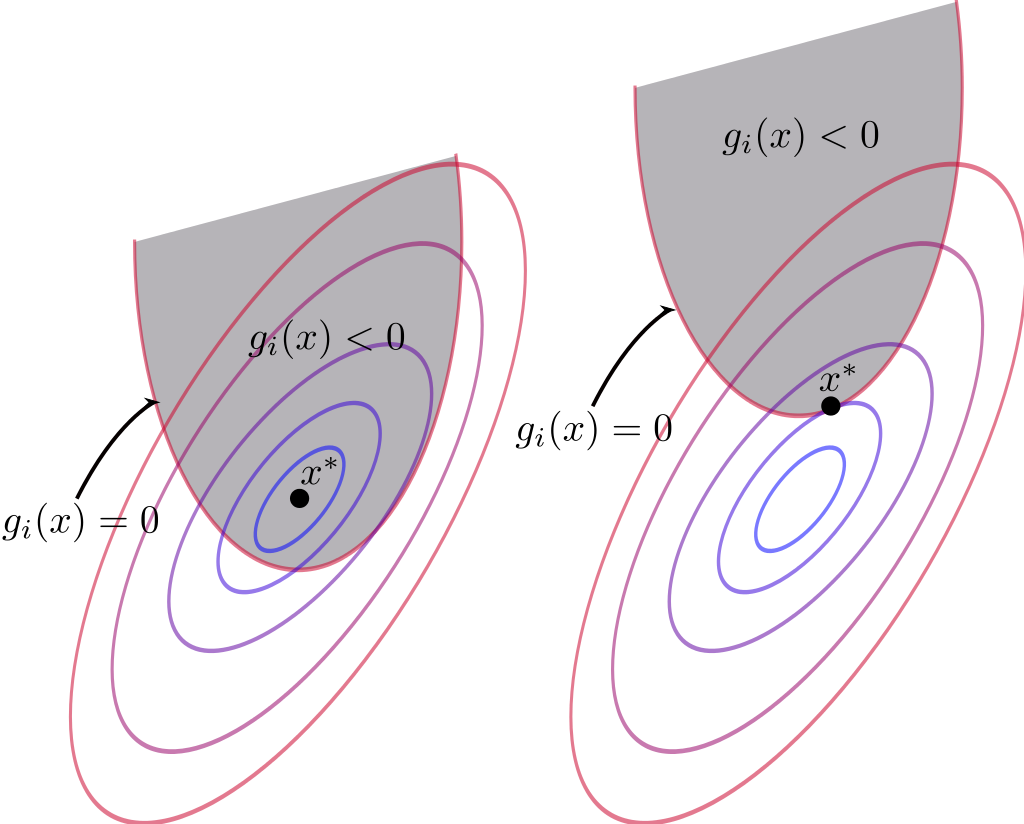
\includegraphics[width=0.5\linewidth]{figures/KKT-IECD}  %插入的图,包括JPG,PNG,PDF,EPS等,放在源文件目录下
					\caption{不等式约束示意}  %图片的名称
					\label{KKT-IECD}   %标签,用作引用
				\end{figure}
				\clearpage
			\end{description}
			\item others
			\begin{itemize}
				\item 一个n阶方块矩阵A的行列式可直观地定义如下:
				$$
				\operatorname{det}(A)=\sum_{\sigma \in S_{n}} \operatorname{sgn}(\sigma) \prod_{i=1}^{n} a_{i, \sigma(i)}
				$$
				${\displaystyle \operatorname {sgn}(\sigma )}$表示置换$ {\displaystyle \sigma \in S_{n}} $的符号差,具体地说,满足 ${\displaystyle 1\leq i\leq j\leq n}$但 ${\displaystyle \sigma (i)>\sigma (j)}$的有序数对${\displaystyle \left(i,j\right)} $称为$\sigma $的一个逆序。如果$ \sigma$ 的逆序共有偶数个,则 ${\displaystyle \operatorname {sgn} \sigma =1} $,如果共有奇数个,则 ${\displaystyle \operatorname {sgn} \sigma =-1} $。
				\item 行列式等于0,矩阵不可逆。
			\end{itemize}
			
			\color{black}
			\item 准确率高达96\%+的模型在真是数据上却完全没法用,可能的原因是什么?
				\begin{itemize}
					\item 数据集不均衡,比如二分类中正样本占了96\%+以上
						如果我们认为真实的数据分布应该是均衡的,那么我们可以采用的解决方法有:
						\begin{description}
							\item[欠采样:] 从样本较多的类中再抽取,仅保留这些样本点的一部分;
							\item[过采样:] 复制少数类中的一些点,以增加其基数;
							\item[生成合成数据:] 从少数类创建新的合成点,以增加其基数。
							\\上述方法都属于重采样,但当训练数据本身并无获取错误时,重采样改变了数据真实的比例,因此要慎重使用;
							\item[添加额外特征] 在数据集中添加一个或多个其他特征,使数据集更加丰富,从而帮助分类。
							\item[重新定义问题] 比如提高少量样本的损失权重
						\end{description}
					\item 模型过拟合
				\end{itemize}
			\item 常用损失函数及激活函数
		\end{enumerate}

	\begin{figure}[H]
		\centering
		\noindent\makebox[\textwidth][c] {
			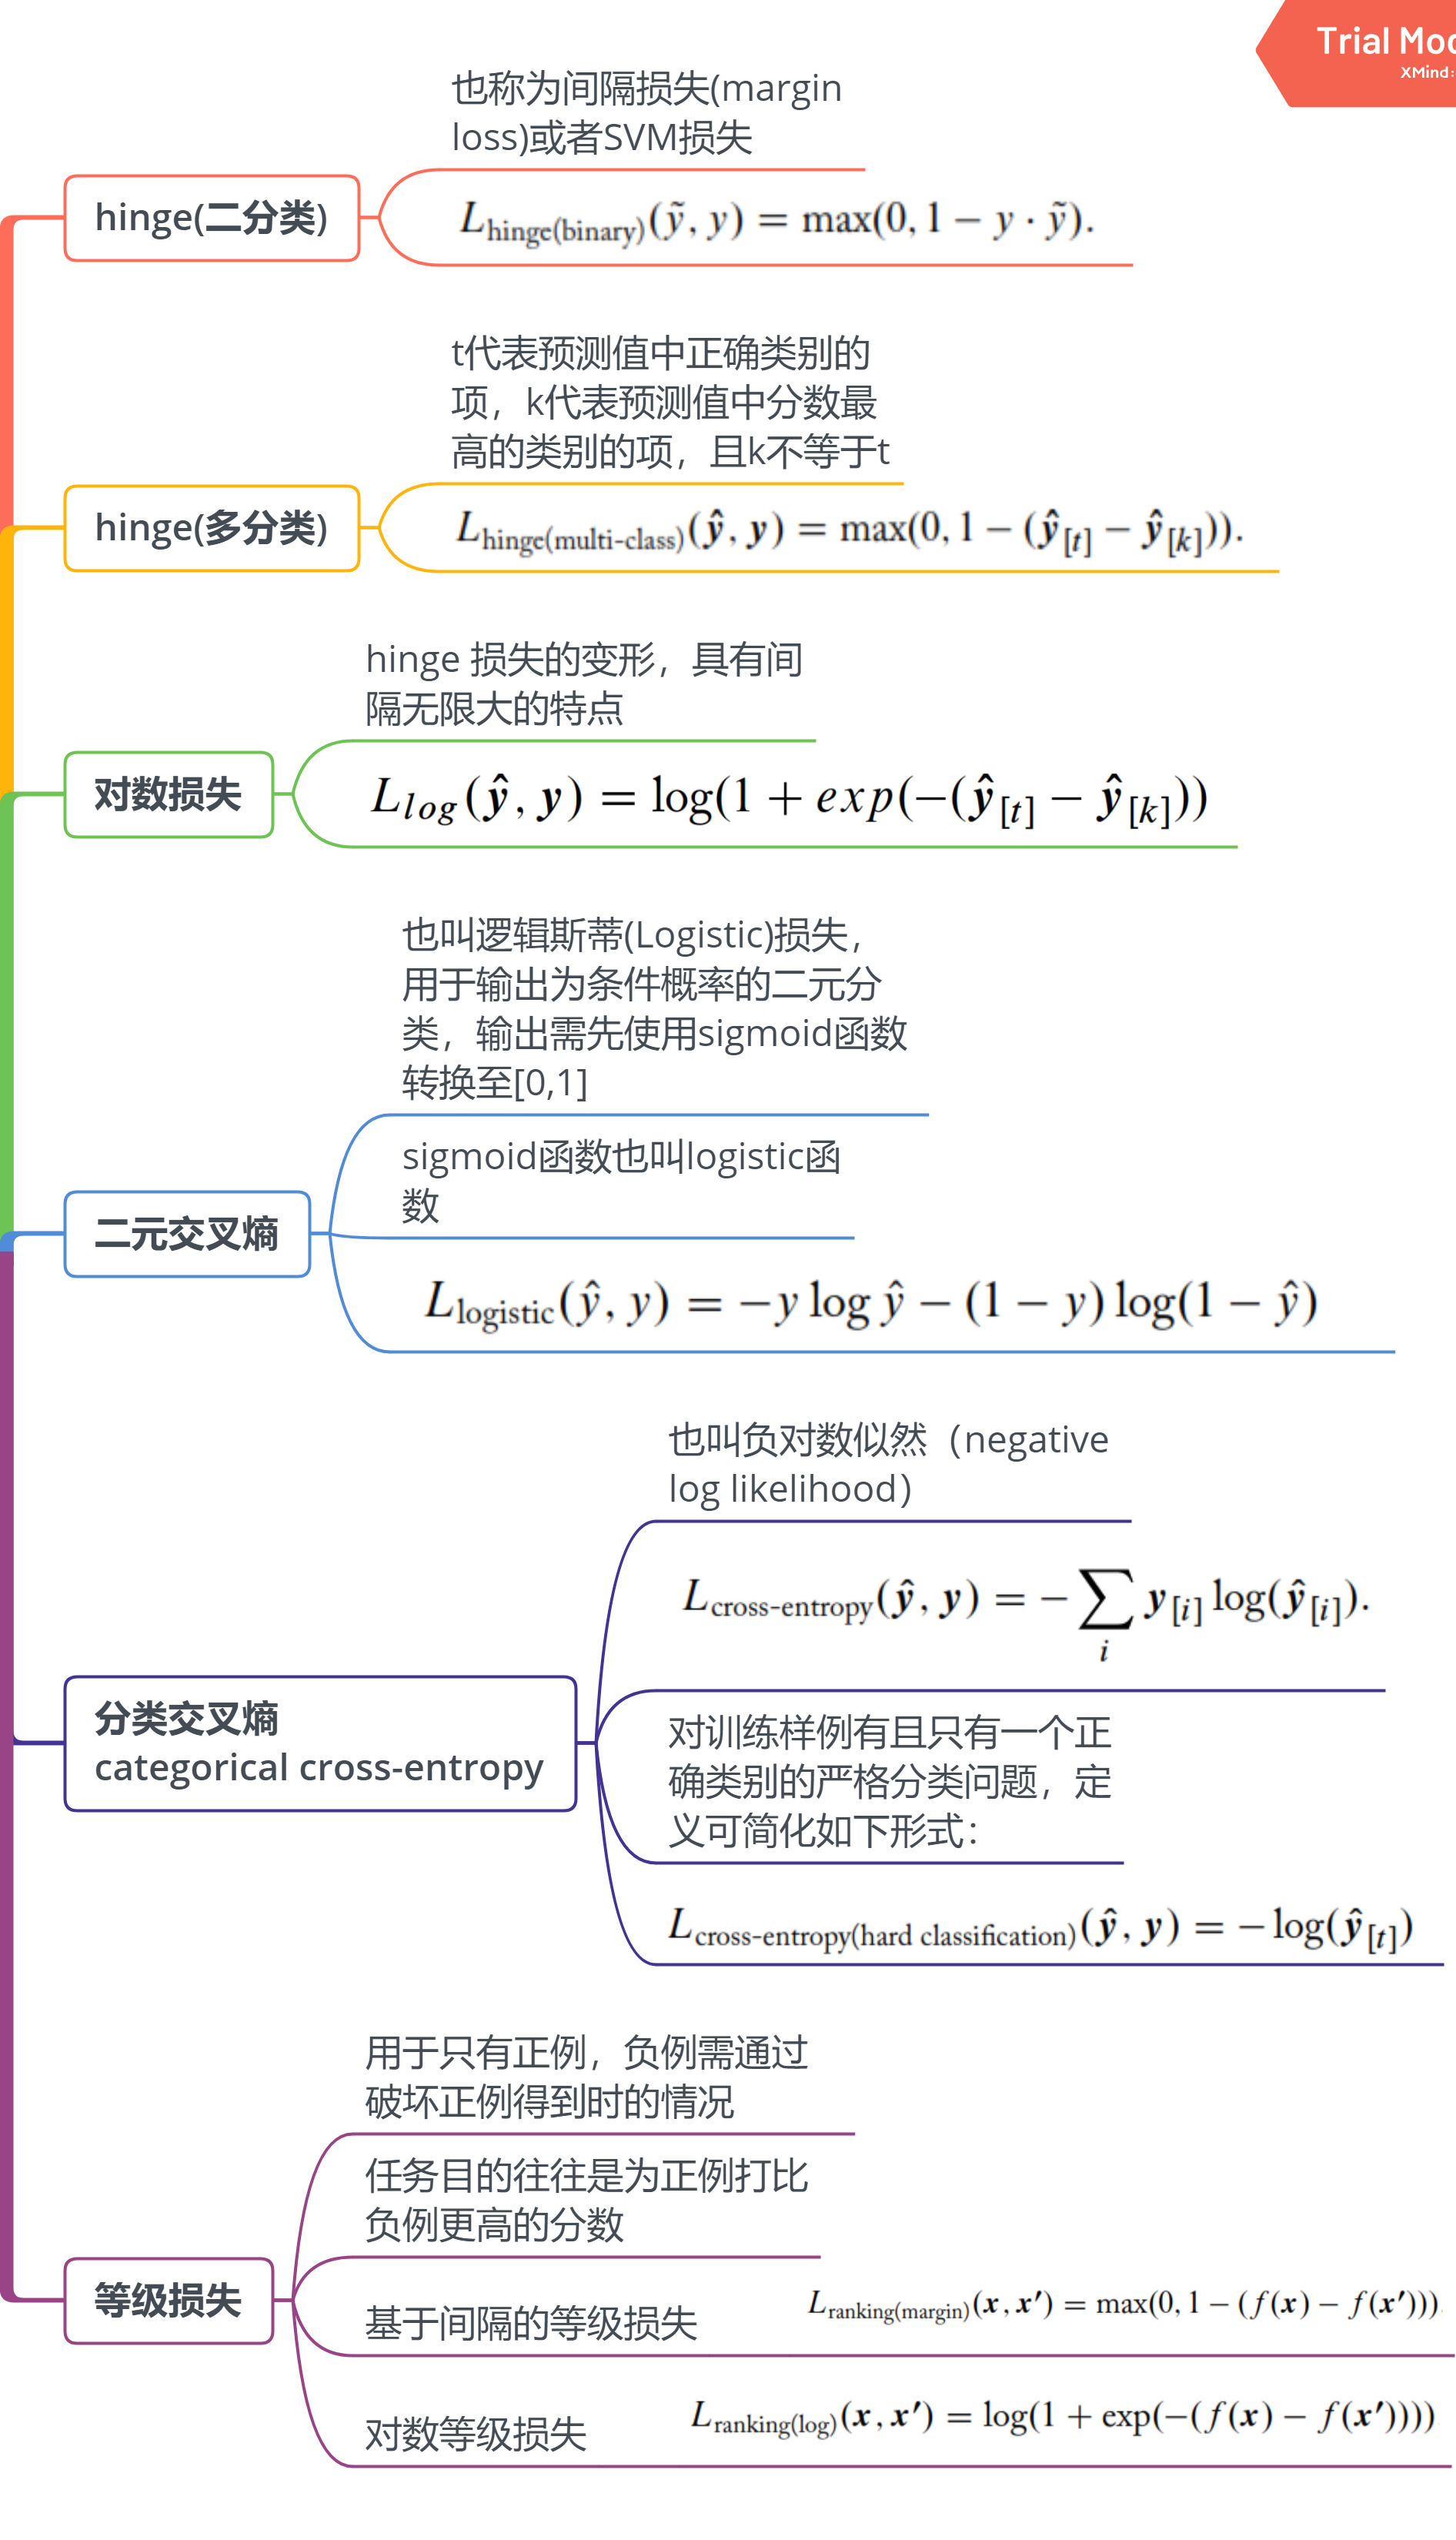
\includegraphics[width=0.55\paperwidth]{figures/lossFunction.png}}
			\caption{LossFunction}  %图片的名称
			\label{LossFunction}   %标签,用作引用
	\end{figure}
	\clearpage
	\begin{figure}[h]%%图
		\centering  %插入的图片居中表示
		\noindent\makebox[\textwidth][c] {
			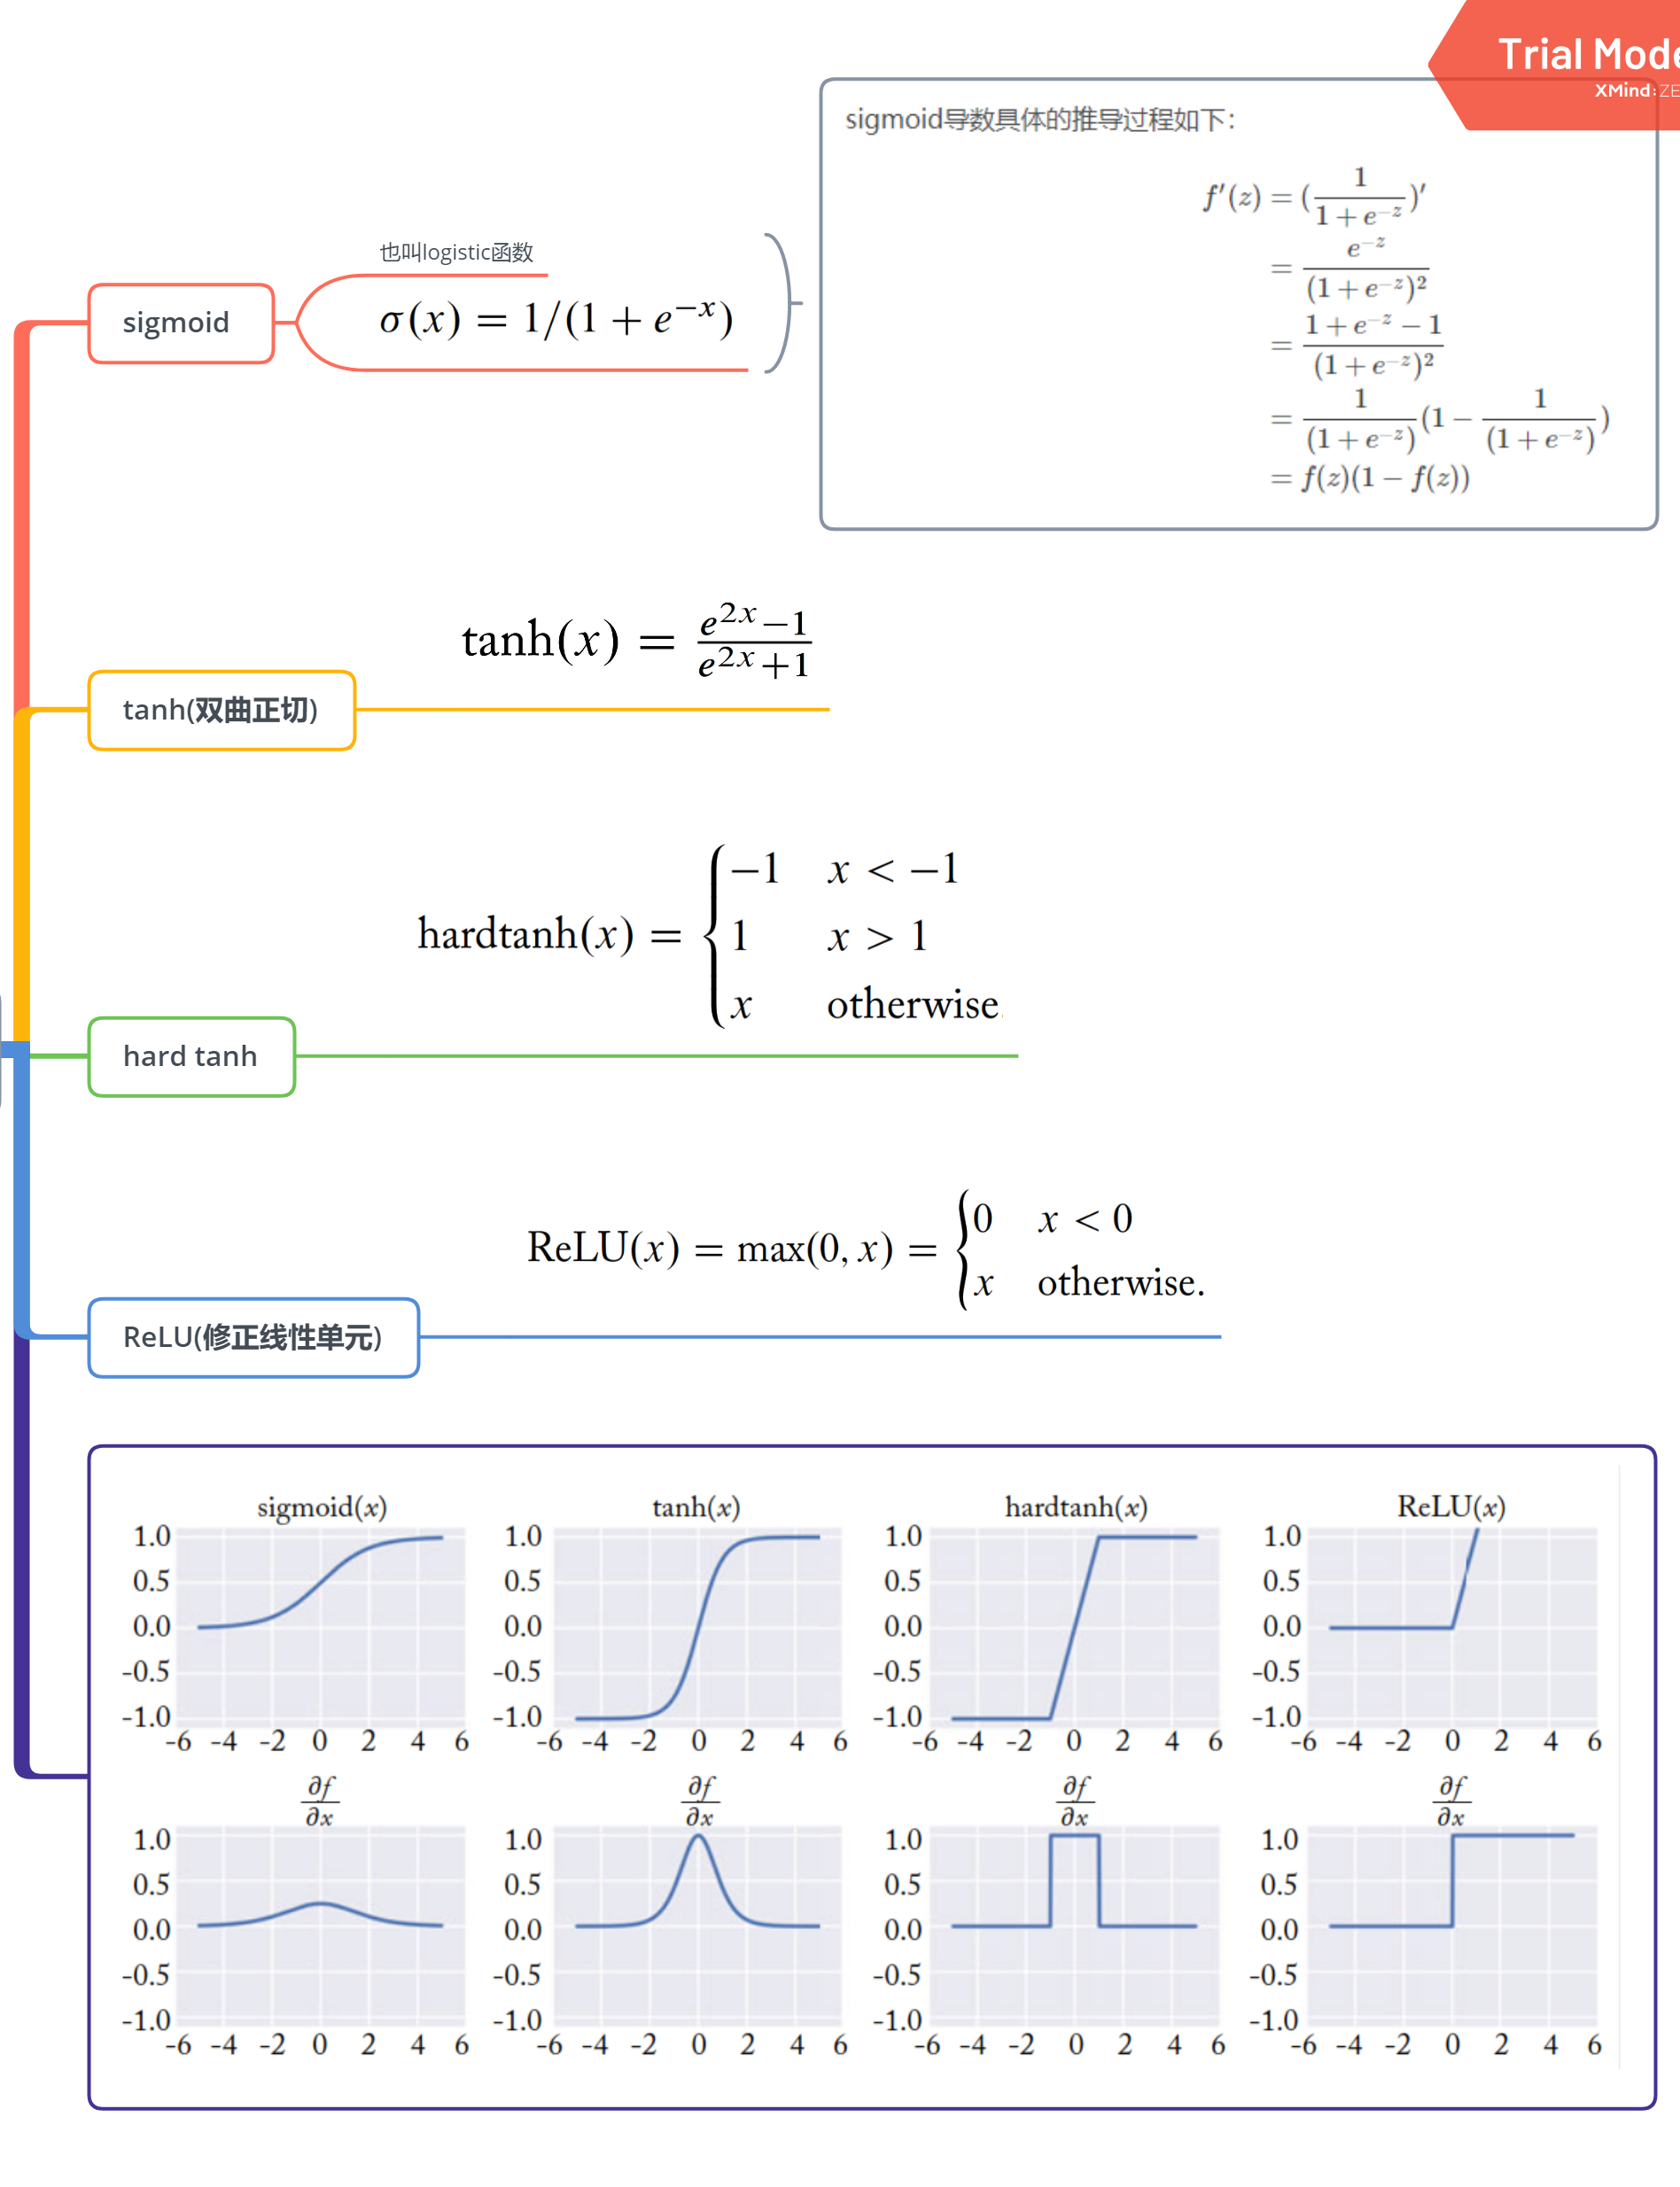
\includegraphics[width=0.75\paperwidth]{figures/ActivationFunction}	}%插入的图,包括JPG,PNG,PDF,EPS等,放在源文件目录下
			\caption{ActivationFunction}  %图片的名称
			\label{ActivationFunction}   %标签,用作引用
	\end{figure}
	\clearpage
	\newpage
	\subsection{迁移学习}
		\begin{enumerate}
			\item 迁移学习:将一个针对其他问题训练好的模型通过简单的调整用于一个新的问题;
			\item 使用方法举例:
			\begin{itemize}
				\item 将AlexNet/Vggnet卷积层的最后一层拿出来,使用SVM或者LR进行分类;
				\item 也可以将多个网络的卷积层的最后输出拿出来进行组合,再用分类器进行分类
				\item 网络越靠后,信息越global,越靠前,越local,local的信息是多数情况共享的(边缘,角度特征),而global的信息和原图紧密相关
			\end{itemize}
			\item 迁移学习的种类
			\begin{itemize}
				\item 同构空间下基于实例的迁移学习;
				\item 同构空间下基于特征的迁移学习;
				\item 异构空间下的迁移学习。
			\end{itemize}
			\item fin-tuning: 利用原有模型的参数信息,作为我们要训练的新的模型的初始化参数,这个新的模型可以和原来一样也可以增添几个层
			\begin{itemize}
				\item 例子:在Alexnet的基础上,我们重新加上一个层再去训练网络,比如再加入一个全连接层,然后先固定前面的层,让新加的fc层的loss值降低到一个很低的值,再调低学习率,放开所有层一块去训练这样可以收敛到一个不错的效果。
			\end{itemize}
		\end{enumerate}
	\newpage
	\section{特征工程}
	\begin{enumerate}
	\item 特征归一化的意义
	\begin{itemize}
	对数值型特征而言:
		\item 消除特征之间量纲的影响,使不同的指标之间具有可比性
		\item 加快模型的训练速度
		\item 常用的方法:
		\begin{description}
			\item [·]线性归一化$X_{norm}=\frac{X-X_{min}}{X_{max}-X_{min}}$
			\item [·]0均值归一化,将原始数据映射到0均值,1方差的标准分布上$z=\frac{x-\mu}{\sigma}$
		\end{description}
		\item 归一化不会改变样本在特征x上的信息增益,因此对于决策树模型归一化不起作用
	\end{itemize}
	\item 对类别性特征,对大多数模型来讲需要将其转换成数值型特征:
	\begin{itemize}
		\item [2.1] 类别型特征编码:
		\item 序号编码
		\item 独热编码,维度较多时需要注意的问题
		\begin{description}
			\item[\#] 可以用向量的稀疏表示节省空间
			\item[\#] 需要配合特征选择来降低维度,原因:\\
				*在k近邻算法中,高维空间中两点之间的距离难以有效衡量\\
				*在逻辑回归模型中,参数量会随着维度增高而增加,容易产生过拟合;\\
				*通常只有部分维度对分类、预测有帮助\\
			\item 编号后准化为二进制编码
		\end{description}
	\end{itemize}

	\item 什么是组合特征?如何处理高维组合特征?
	\begin{itemize}
		\item 组合特征的作用:
			a.提高数据对复杂关系的拟合能力\\
		\item 一种特征组合方式\\
			a.构造决策树,决策树根节点到叶节点的每条都可以看做一种特征组合方式
	\end{itemize}
	\item 对于分类任务,数据量不足导致的主要问题在于过拟合
	\item 降低过拟合风险的措施:
		\begin{itemize}
			\item 针对模型:简化模型、添加约束(如正则化)、集成学习、DropOut超参数
			\item 针对数据,图像数据可以采用平移、旋转、添加噪声等手段生成新的数据
		\end{itemize}
	\end{enumerate}
	\newpage
	\section{模型评估及优化}
		1.两个阶段:离线评估、在线评估\\
		2.指标:准确率(Accuracy)、精确率(Precision)、召回率(recall)、均方根误差(RMSE)\\
		\subsection{准确率的局限性}
		
		$$Accuracy=\frac{n_{correct}}{n_{total}}$$
		当数据不均衡时,占比例大的类别会成为影响准确率的主要因素。如负样本占99\%时,简单的将所有数据都判断为负样本即可获得99\%的准确率.\\
		替代方案可以选择使用每个类别的样本准确率的算术平均代替准确率。
		
		\subsection{精确率与召回率的权衡}
		$$precision=\frac{n_{truepositive}}{n_{positive}}$$
		$$recall=\frac{n_{truepositive}}{n_{true}}$$
		在排序问题中,P-R曲线为阈值从高到低是pre和recall的变化曲线,曲线的整体变化能够对模型做出更全面的评估,由此引出了F1值,它是pre和recall的调和平均。
		$$F1=\frac{2*pre*recall}{pre+recall}$$
		
		\subsection{RMSE的“意外”}
		$$RMSE=\sqrt\frac{\sum_{i=1}^{n}(y-\hat{y})^2}{n}$$
		\begin{enumerate}
			\item回归模型的预测误差不大,但RMSE却很大,可能的原因:
			\begin{itemize}
				\item[\#] 离群点,解决方案:
					\item 过滤“离群点”
					\item 部分“噪声点”可能并不是“离群点”,那么就需要建模处理这种情况的机制;
					\item 使用比RMSE更鲁棒的指标:平均绝对百分比误差(MAPE)
				$$MAPE=\sum_{i=1}^{n}\left|\frac{y_i-\hat{y_i}}{n}\right|\times\frac{100}{n}$$
			\end{itemize}
		\end{enumerate}
	
		\subsection{ROC曲线}
		Receiver Operating Characteristic Curve
		\begin{enumerate}
			\item 横坐标,假阳性率:FPR=FP/N
			\item 纵坐标,真阳性率:TPR=TP/P
			\item AUC,ROC曲线下面积,反映了模型的性能
			\item ROC曲线相对于P-R曲线的特点:
				\begin{itemize}
					\item 当正负样本的分布发生变化时,ROC曲线能够基本保持不变,但P-R曲线一般会剧烈变化
					\item 但P-R曲线能够更好的反应模型在特定数据集上的性能
				\end{itemize}
		\end{enumerate}
	
		\subsection{余弦距离}
		\subsection{模型评估的方法}
			\begin{enumerate}
				\item 模型评估过程中的验证方法及其优缺点
				\begin{itemize}
					\item Hlodout检验:将原始样本集随机划分为训练集和测试集两部分
					\begin{description}
						\item[缺点] 验证结果和原始数据划分有很大关系
						\item[解决方法] 交叉验证:k-fold,留一验证;自助法:进行n次又放回的随机抽样得到训练集,未被抽到过的样本作为验证集
					\end{description}
				\end{itemize}
			\end{enumerate}
	\begin{enumerate}
		\item 余弦距离是归一化的,衡量向量夹角,不受数据维度影响
		\item 欧氏距离数值受维度影响较大
		\item 余弦距离反应相对距离,关注数值绝对差异时应使用欧氏距离
		\item 严格定义的距离应该满足的条件
		\begin{itemize}
			\item 正定性
			\item 对称性
			\item 三角不等式$dist(A,B)+dist(B,C)>dist(A,C)$
		\end{itemize}
	\end{enumerate})
	
		\subsection{超参数调优}
		\begin{enumerate}
			\item 网格搜索
			\begin{itemize}
				\item 采用较大的范围和较小的步长,很有可能得到全局最优,但开销巨大
				\item 加大步长能加速搜索,但可能由于目标函数的非凸性导致错过全局最优解
			\end{itemize}
			\item 随机搜索
			\begin{itemize}
				\item 在选定的搜索范围中随机选取样本点
				\item 也是无法保证找到全局最优
			\end{itemize}
			\item 贝叶斯优化算法
			\begin{itemize}
				\item 根据先验分布,假设一个搜集函数,在优化过程中不断使用新的采样点对目标函数进行测试并更新其先验分布;最后,算法测试由后验分布给出的最可能的全局最优解。
				\item 一旦进入局部最优容易陷入
				\item "探索"(在未采样区域采样)和"利用"(利用后验分布在最可能的区域采样)结合解决局部最优问题。
			\end{itemize}
		\end{enumerate}	
		
		\subsection{过拟合与欠拟合}
		\begin{enumerate}
			\item 过拟合:在训练集上表现很好但在测试集和新数据上表现较差
			\item 如何降低过拟合和欠拟合
			\begin{itemize}
				\item 对于过拟合
				\begin{description}
					\item[*] 获得更多的训练数据
					\item[*] 降低模型复杂度(神经网络减少层数、决策树规约及剪枝等)
					\item[*] 正则化方法
					\item[*] 集成学习方法
				\end{description}
				\item 对于欠拟合
				\begin{description}
					\item[*] 添加新特征
					\item[*] 增加模型复杂度
					\item[*] 降低正则化系数
				\end{description}
			\end{itemize}
		\end{enumerate}
		\subsection{初始化参数方法}
		例如Xavier初始化
		\subsection{batch normalization}
			\begin{enumerate}
				\item  Internal Covariate Shift(在深层网络训练的过程中,由于网络中参数变化而引起内部结点数据分布发生变化的这一过程)问题解决办法
				\begin{itemize}
					\item 白化(Whitening)
						\begin{description}
							\item[目的]使得输入特征分布具有相同的均值与方差以及去除特征之间的相关性。
							\item[a.] PCA白化:保证了所有特征分布均值为0,方差为1;
							\item[b.] ZCA白化保证了所有特征分布均值为0,方差相同;
							\item[存在的问题] 计算成本太高;改变了网络每一层的分布,因而改变了网络层中本身数据的表达能力。
						\end{description}
					\item batch normalization算法思想:在每个mini-batch上进行两部分操作:
						\begin{description}
							\item[a1.] 对每个特征(每一维)单独进行normalization,使得每个特征的均值为0,方差为1;
							\item[a2.] 在每一层进行normalization后再加一个线性变换以恢复每层数据的表达能力。
						\end{description}
					\item 算法步骤
						\begin{description}
							\item[normalization] $$\mu_j=\frac{1}{m}\sum_{i=1}^{m}Z_j^{(i)}$$ $$\delta_j^2=\frac{1}{m}\sum_{i=1}^{m}(Z_j^{(i)}-\mu_j)$$ $$\hat{Z_j}=\frac{Z_j-\mu_j}{\sqrt{\delta_j^2+\epsilon}}$$
							其中$\epsilon$是为了防止方差为0的平滑
							\item [可学习参数: ] 为了恢复数据本身的表达能力,引入可学习参数$\gamma,\beta$对规范化后的数据进行线性变换$\tilde{ Z_j}=\gamma_j\hat{Z_j}+\beta_j$,记为$$A_j=g(\tilde{ Z_j})$$特别的,当$\gamma=\delta^2,\beta=\mu$时可实现等价变换并且保留原始输入特征的分布。
							\item[P.S.]由于进行normalization时会减去均值,在整个BN过程中可以忽略偏置项$b$或者将其置为0
						\end{description}
					\end{itemize}
				\item 测试时BN的用法
				\begin{itemize}
					\item 使用所有batch训练数据的$\mu$和$\delta^2$的期望对测试数据进行normalization
					\item 也可以对训练阶段每个batch的$\mu$和$\delta^2$做加权平均得到测试阶段是使用的$\mu$和$\delta^2$
				\end{itemize}
				\item 优点
				\begin{description}
					\item[a.] BN使得网络中每层输入数据的分布相对稳定,加速模型学习速度
					\item[b.] BN使得模型对网络中的参数不那么敏感,简化调参过程,使得网络学习更加稳定
					\item[c.] BN允许网络使用饱和性激活函数(例如sigmoid,tanh等),缓解梯度消失问题
					\item[d.] BN具有一定的正则化效果
				\end{description}
			\end{enumerate}
		\subsection{SGD}
		
		\subsection{AdaGrad}
		(1)从AdaGrad算法中可以看出,随着算法不断迭代,r会越来越大,整体的学习率会越来越小。所以,一般来说AdaGrad算法一开始是激励收敛,到了后面就慢慢变成惩罚收敛,速度越来越慢。

	\newpage
	\section{采样}
		作用:
		\begin{enumerate}
			\item 将复杂的分布简化为离散的样本点,从某种程度上可以看做一种信息降维
			\item 可以用重采样对样本集进行调整以更好的适应后期的模型学习
			\item 可以用于随机模拟以进行复杂模型的近似求解或推理
			\item 重采样:
				\begin{itemize}
					\item 自助法
					\item 刀切法
					\item 在保持特征的信息下,有意识的改变样本分布,以适应后续的模型训练和学习;例如对不均衡的训练样本进行重采样
				\end{itemize}
			\item 生成均匀分布的随机数
				\begin{itemize}
					\item 计算机只能生成离散的且并非完全随机的伪随机数,连续分布通过在较大的离散空间上进行逼近。
					\item 线性同余法(Linear Congruential Generator)(LCG)$$x_{t+1}\equiv (a \bullet x_t +c)\mod m$$其中$x_0$称为随机数种子。
					\item 一个好的线性同余随机数生成器要让其循环周期尽量接近m
					\item 待解决的问题:
					\begin{description}
						\item[线性同余法中的随机种子一般如何选定?]
						\item[如果要产生高维或大量样本,LCG存在什么问题?]
						\item[如何证明上述算法得到的随机数序列可以近似均匀分布?]  
					\end{description}
				\end{itemize}
			\item 常见的采样方法:
			\begin{itemize}
				\item 
			\end{itemize}	
		\end{enumerate}
	\newpage
	\section{词向量}
		\subsection{word2vec}
		\subsection{fastText}
		\subsection{GloVec:Global Vectors for Word Representation}
		1.根据语料库(corpus)构建一个共现矩阵(Co-ocurrence Matrix)X,矩阵中的每一个元素$X_{ij}$代表单词
		i和上下文单词j在特定大小的上下文窗口(context window)内共同出现的次数,但并不是简单的计算共现次数,而是在其基础上使用衰减函数$decay=1/d$,也就是说距离越远的两个单词所占总计数(total count)的权重越小。\\
		
		2.构建词向量(Word Vector)和共现矩阵(Co-ocurrence Matrix)之间的近似关系:
		$$w_{i}^{T}\tilde{w_{j}} + b_i + \tilde{b_j} = \log(X_{ij}) $$ \label{1-1}
		推导:略\\
		3. 构建损失函数(mean square loss with $f(X_{ij}$):$$J = \sum_{i,j=1}^{V} f(X_{ij})(w_{i}^{T}\tilde{w_{j}} + b_i + \tilde{b_j} – \log(X_{ij}) )^2 $$ \label{1-2}
		$f(X)_{ij}$的作用:\\
		a.共现次数多的单词的$X_{ij}$的权重大,但权重也要有上限\\
		b.未共现的单词的$X_{ij}$的权重应为0\\
		原文采用的形式:
		\begin{equation} 
		f(x)=\begin{cases} 
		(x/x_{max})^{\alpha}  & \text{if} \ x < x_{max} \\ 
		1 & \text{otherwise} 
		\end{cases} 
		\end{equation} \label{1-3}
		\begin{figure}[h]%%图
			\centering  %插入的图片居中表示
			\noindent\makebox[\textwidth][c] {
				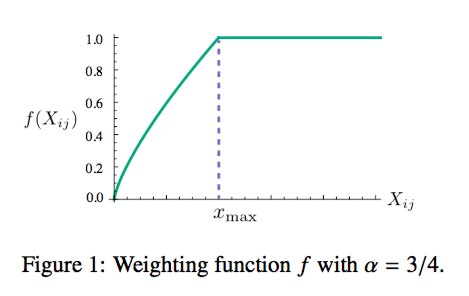
\includegraphics[width=0.33\paperwidth]{figures/GloVec_f_Xij}	}%插入的图,包括JPG,PNG,PDF,EPS等,放在源文件目录下
			\caption{GloVec\_f\_Xij}  %图片的名称
			\label{GloVec_f(Xij)}   %标签,用作引用
		\end{figure}
	
		\subsection{encoder-decoder+seq2seq}
			\href{https://zhuanlan.zhihu.com/p/27608348}{实战从Encoder到Decoder实现Seq2Seq模型}
		\newpage
		\subsection{Attention Is All Your Need: Transformer}
		    \begin{figure}[h]%%图
				\centering  %插入的图片居中表示
				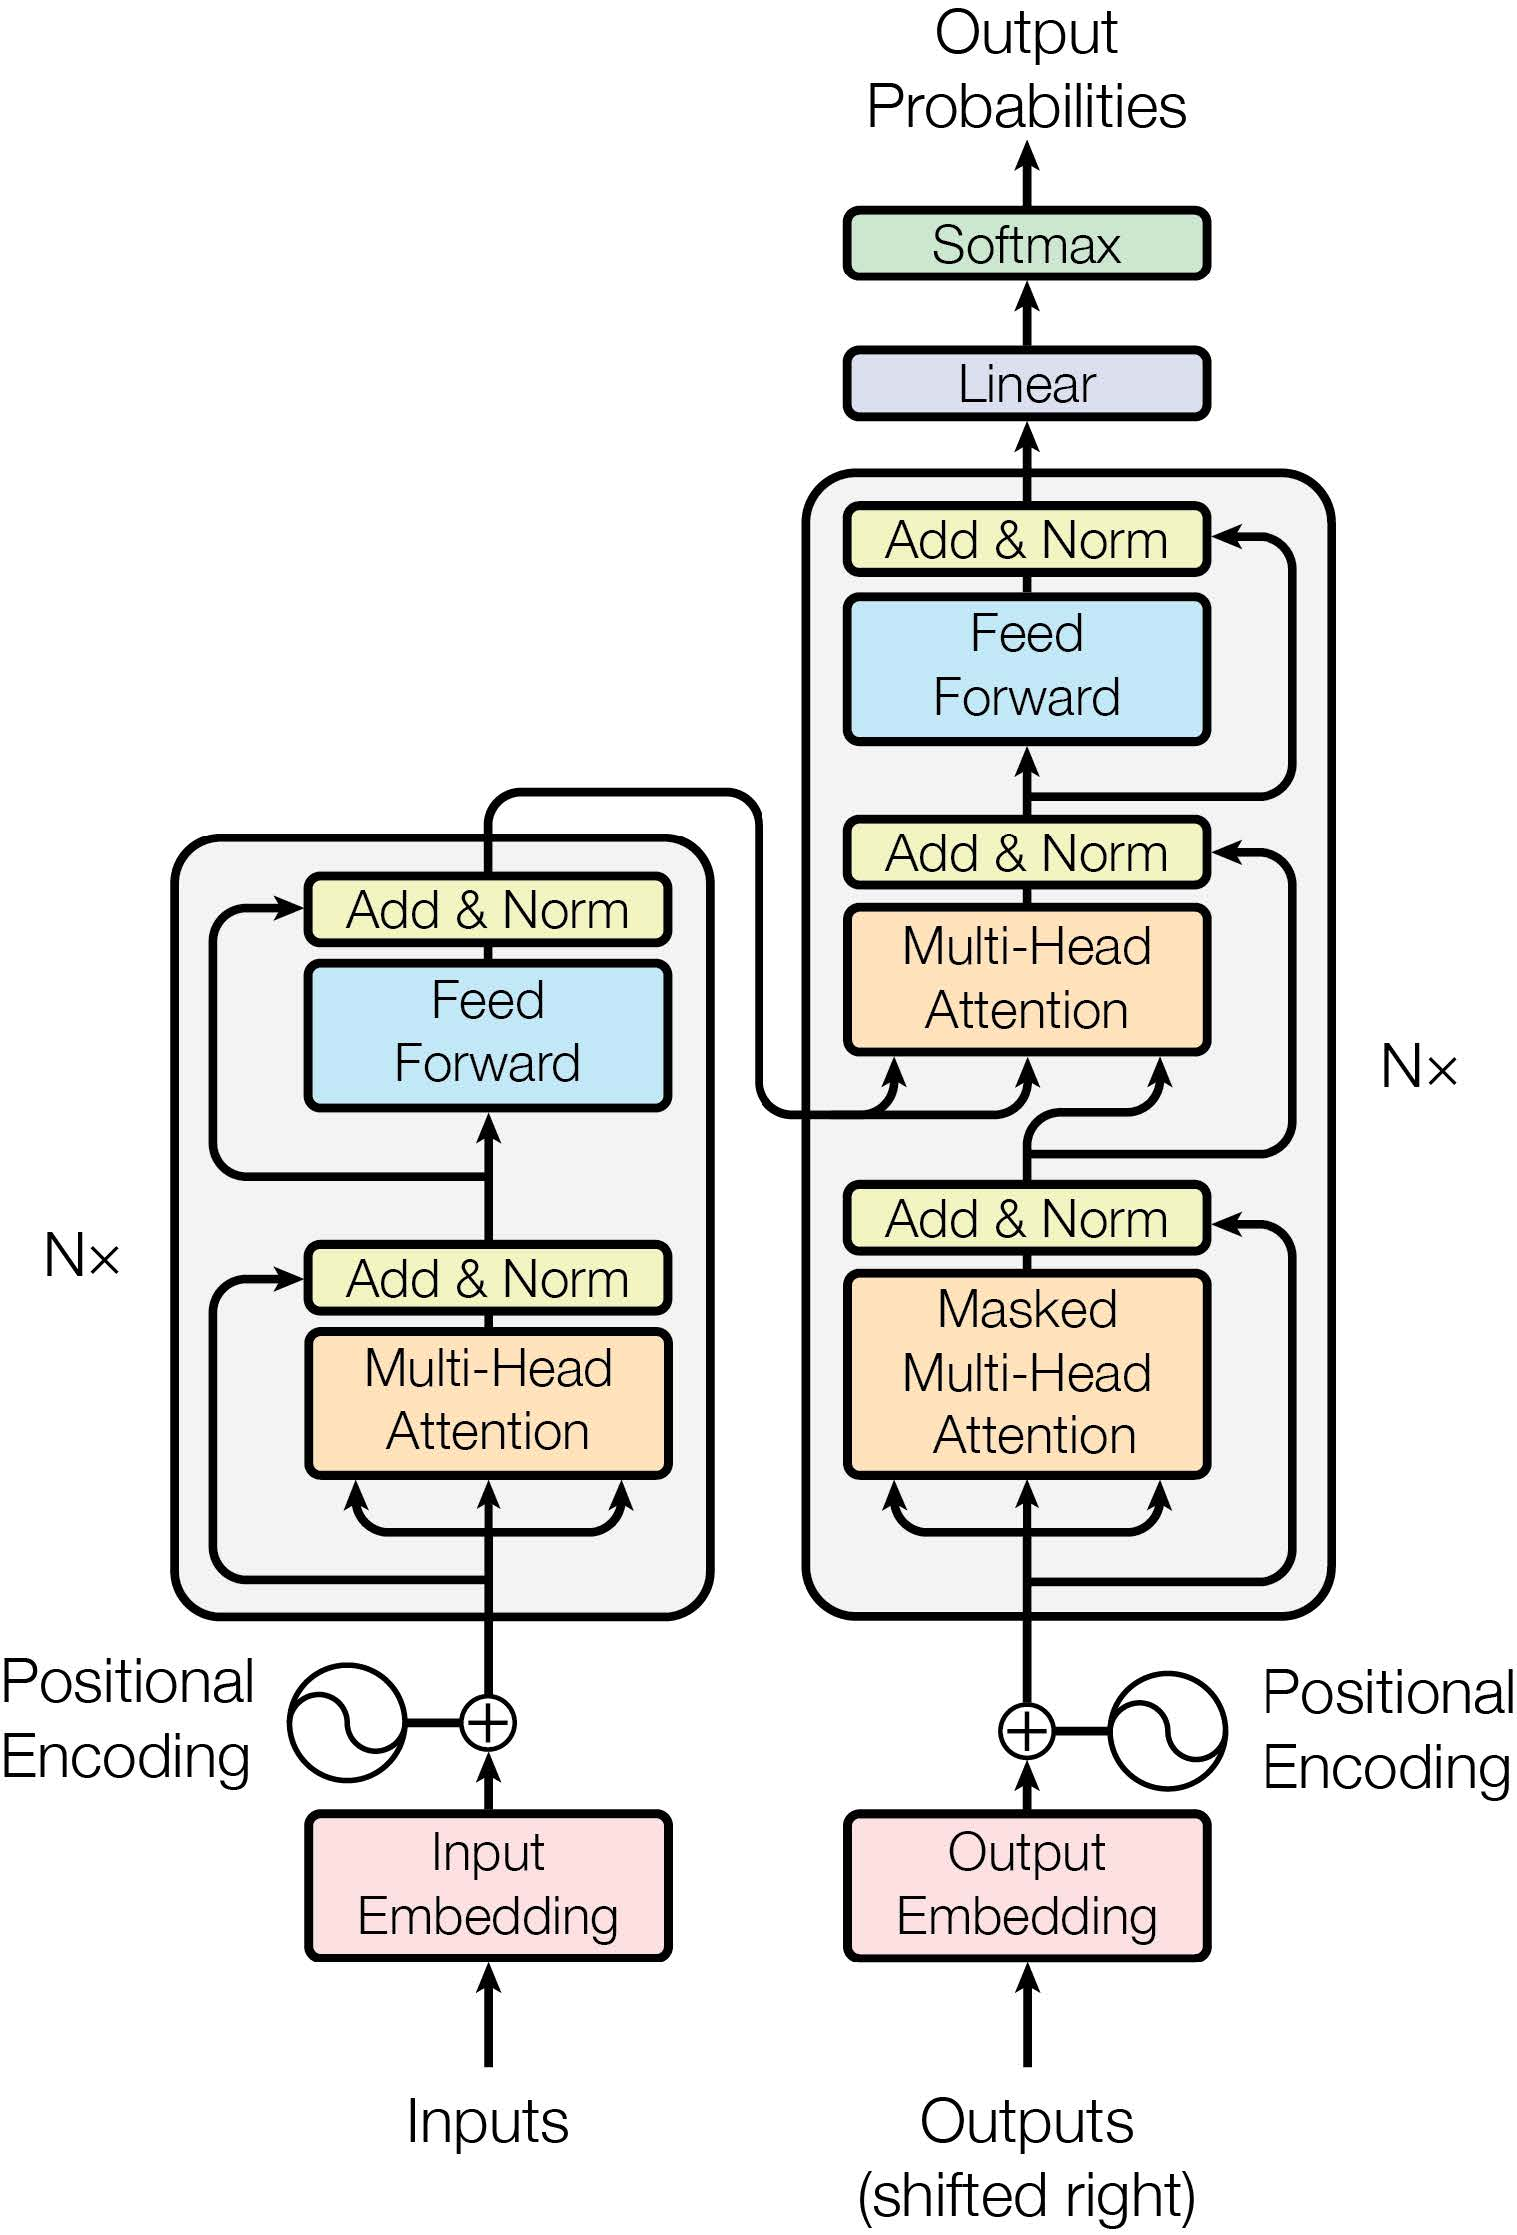
\includegraphics[width=0.5\linewidth]{figures/Transformer}  %插入的图,包括JPG,PNG,PDF,EPS等,放在源文件目录下
				\caption{Transformer}  %图片的名称
				\label{Transformer}   %标签,用作引用
			\end{figure}

			As we all know:$attention\_output=Attention(Q,K,V)$\\
			multi-head attention 是通过h个不同的线性变换对Q,K,V进行投影,最后将不同的attention结果拼接起来:
			$$MultiHead(Q,K,V)=Concat(head_1,head_2,...,head_h)W^o$$
			while $head_i=Attention(QW_i^Q,KW_i^k,VW_i^V)$\\
			self-attention就是取Q,K,V相同。
			\begin{enumerate}
				\item Attention Is All You Need
				\begin{itemize}
					\item \href{https://arxiv.org/pdf/1706.03762.pdf}{论文地址}
					\item \href{https://github.com/Kyubyong/transformer}{Tensorflow}
					\item \href{https://github.com/jadore801120/attention-is-all-you-need-pytorch}{pytorch}
				\end{itemize}
				\item 1.没有采取大热的RNN/LSTM/GRU的结构,而是使用attention layer,达到了较好的效果,并且解决了RNN/LSTM/GRU 里的long dependency problem
				\item 2.masking 的作用就是防止在训练的时候使用未来的单词作为输出。
			\end{enumerate}
			attention可能存在的问题以及解决方案:
			\begin{enumerate}
				\item 可能存在的问题1.
				\begin{itemize}
					\item 输入句子过长的话会导致attention map过大,内存爆炸
					\item 可行的解决方案:
					\begin{description}
						\item[a.] 减小batch size 并使用多gpu训练
						\item[b.] 对K,V做卷积,降低每一行的维度
					\end{description}
				\end{itemize}
			\end{enumerate}
				\subsection{模型对比}
		\begin{figure}[h]%%图
			\centering  %插入的图片居中表示
			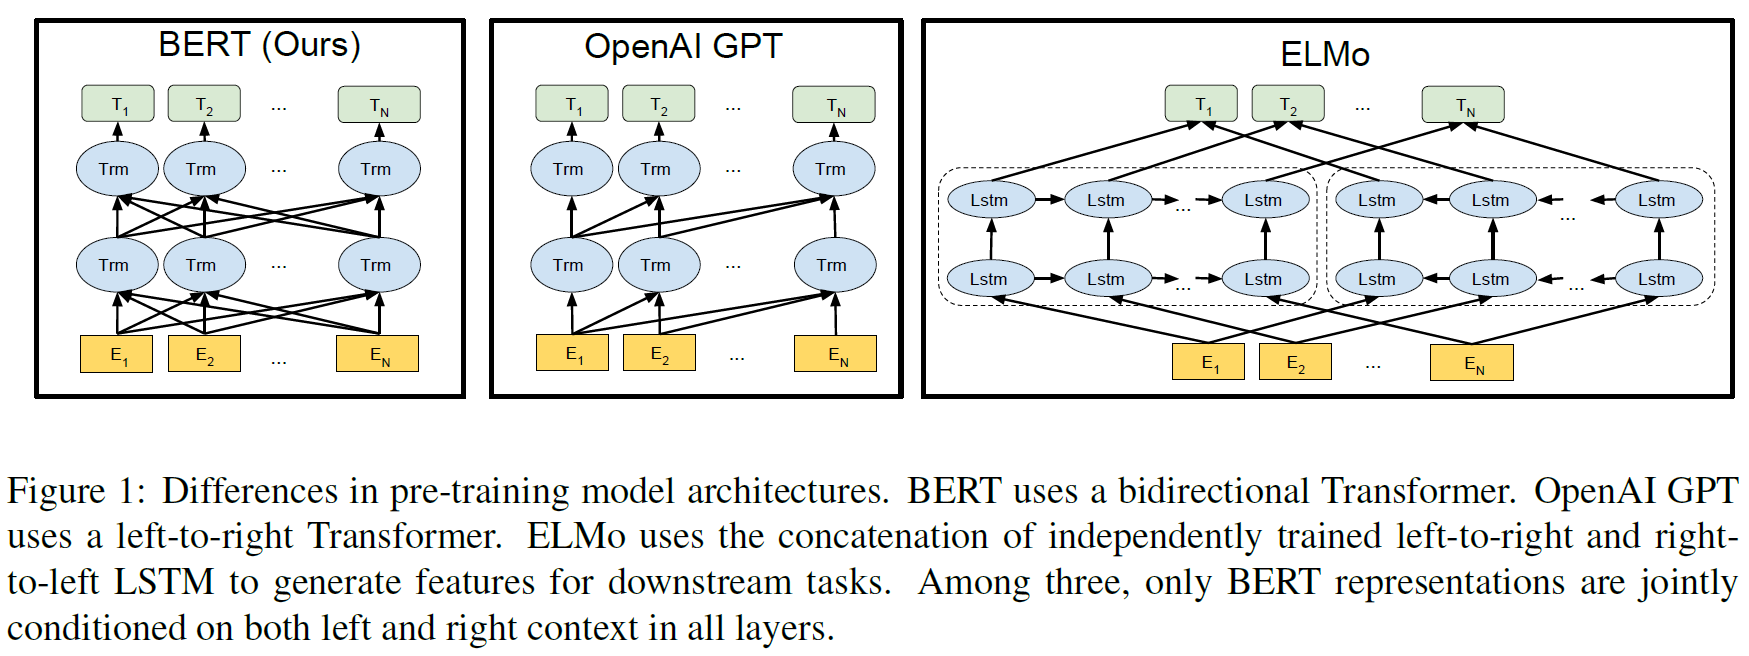
\includegraphics[width=1.0\linewidth]{figures/elmo-gpt-bert}  %插入的图,包括JPG,PNG,PDF,EPS等,放在源文件目录下
			\caption{elmo VS gpt VS bert}  %图片的名称
			\label{elmo-gpt-bert}   %标签,用作引用
		\end{figure}
		\subsection{Elmo:Embedding from Language Models}
		
		\begin{enumerate}
			\item 使用双层双向RNN预训练
			\item 语言模型作为训练任务
			\item 对于每个词,生成三个词向量——单词特征、句法特征、语义特征
		\end{enumerate}
		\subsection{GPT:Generative Pre-Training}
		
		\begin{enumerate}
			\item 使用transformer(encoder部分)替代Elmo中的RNN,构建了新的模型。
		\end{enumerate}
		\subsection{Bert:Bidirectional Encoder Representations from Transformers}
		\begin{enumerate}
			\item 优点
			\begin{itemize}
				\item[a.] 效果好,这是最大的优点 
				\item[b.] 捕捉到的是真正意义上的bidirectional context信息
				\item[c.] 用的是Transformer,也就是相对rnn更加高效、能捕捉更长距离的依赖。
			\end{itemize}
			\item 缺点
			\begin{itemize}
				\item[a.] [MASK]标记在实际预测中不会出现,训练时用过多[MASK]影响模型表现
				\item[b.] 每个batch只有15\%的token被预测,所以BERT收敛得比left-to-right模型要慢
			\end{itemize}
		\end{enumerate}
	\newpage
	\section{主题模型}
	\subsection{LSI/LSA}
		LSI(Latent semantic indexing, 潜语义索引)和LSA(Latent semantic analysis,潜语义分析)指的是同一种方法;\\
		LSA 使用向量来表示词(terms)和文档(documents),并通过向量间的关系(如夹角)来判断词及文档间的关系; 将词和文档映射到潜在语义空间,从而去除了原始向量空间中的一些“噪音”,提高了信息检索的精确度。
		\begin{enumerate}
			\item 构建词-文档(term-document)共现矩阵$M_{TD}$
			\item 对M进行奇异值分解(SVD)得到$M=UDV^T$,分解完的奇异值矩阵中有奇异值不均衡的特点,我们选取奇异值较大的部分及其对应的奇异向量
			\item 选取后得到矩阵$X_{TC}B_{CC}Y_{CD}$,其中
				\begin{itemize}
					\item$X_{TC}$是对词进行分类的一个结果,每一行表示一个词,每一列表示一个语义相近的词类,非零元素表示词和语义类的相关性
					\item $B_{CC}$表示词的类和文章的类之间的相关性
					\item $Y_{CD}$每一行表示一个主题,每一列表示一个文本,非零元素表示文本与主题的相关性
				\end{itemize}
			\item \color{red}LSA 模型通常用 tf-idf 代替文档词频计数	
			\color{black}
			
			优点:
				\begin{itemize}
					\item  通过降维去除了部分噪声,使特征更加“鲁棒”
					\item 充分利用冗余数据
					\item 与语言无关
					\item 无监督,自动化
				\end{itemize}
			缺点:
				\begin{itemize}
					\item 缺乏可解释的嵌入(我们并不知道主题是什么,其成分可能积极或消极,这一点是随机的)
					\item 需要大量的文件和词汇来获得准确的结果
					\item SVD优化目标基于L-2 norm,隐含假设数据服从高斯分布(优化范数),然而现实中数据出现的次数均为非负的,明显与假设不符。
					\item SVD的计算复杂度很高(尤其是当$D$矩阵很大时),不能实现增量学习。
				\end{itemize}	
		\end{enumerate}
	\subsection{PLSA}
	Probability  Latent semantic indexing
		\begin{enumerate}
			\item 建模思想:对于可观测变量建立似然函数,将隐含变量暴露出来,并使用E-M算法求解。其中M步的标准做法是引入Lagrange乘子求解后回代到E步。
			\item 表示方法:
				\begin{itemize}
					\item 给定文档 d,主题 z 以 $P(z|d)$ 的概率出现在该文档中
					\item 给定主题 z,单词 w 以$ P(w|z) $的概率从主题 z 中提取出来
					
				\end{itemize}
			\item 两种模型的表示方法
			\begin{itemize}
				\item 模型表示1:从概率为 $P(d)$ 的文档开始,然后用$ P(z|d) $生成主题,最后用 $P(w|z) $生成单词
				$$P(D,W)=P(D)\sum_{Z}P(Z|D)P(W|Z)$$
				\item 模型表示2:从$ P(z) $开始,再用$ P(d|z) $和 $P(w|z)$单独生成文档。
				$$P(D,W)=\sum_{Z}P(Z)P(D|Z)P(W|Z)$$
			\end{itemize}
			\item 使用EM算法求解pLSA的基本实现方法:
				\begin{itemize}
					\item E步骤:求给定当前估计参数条件下隐含变量的后验概率;
					\item M步骤:最大化Complete data对数似然函数的期望,此时我们使用E步骤里计算的隐含变量的后验概率,得到新的参数值。
					\item E-M迭代进行直到收敛。
				\end{itemize}
			\item 不足
				\begin{itemize}
					\item 没有对 P(D) 建模,所以无法为新文档分配P(D)概率
					\item pLSA 的参数数量随着我们拥有的文档数线性增长,因此容易出现过度拟合问题
					\item pLSA 很少单独使用,一般使用过LSA后会直接尝试LDA
				\end{itemize}
		\end{enumerate}
	
	\subsection{LDA}
	\subsection{lda2vec}
	lda2vec是word2vec的skip-gram模型的扩展;
	lda2vec不仅能学习单词的词嵌入(和上下文向量嵌入),还同时学习主题表征和文档表征。
	
	\newpage
	\section{强化学习}
	\newpage
	\section{集成学习}
		\begin{figure}[h]%%图
			\centering  %插入的图片居中表示
			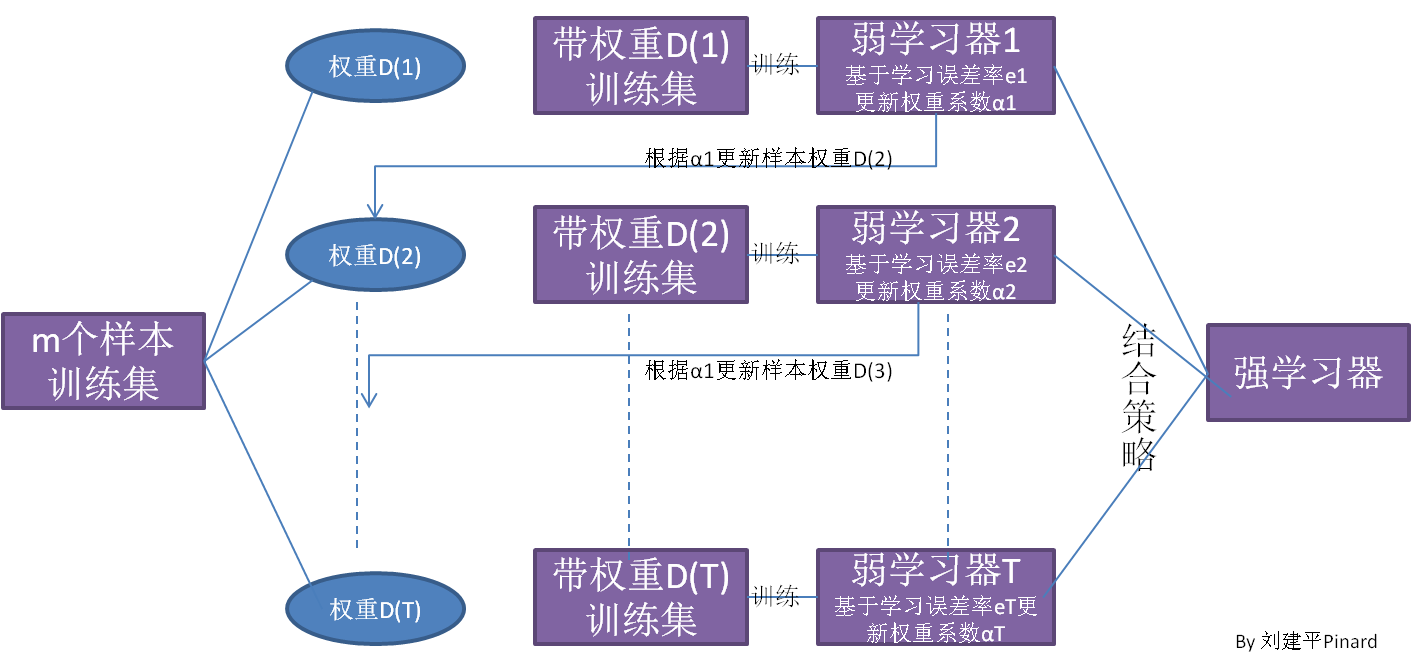
\includegraphics[width=1.0\linewidth]{figures/adaboost}  %插入的图,包括JPG,PNG,PDF,EPS等,放在源文件目录下
			\caption{boosting算法基本思想}  %图片的名称
			\label{boosting}   %标签,用作引用
		\end{figure}
		\subsection{bagging}
		每一次从原始数据中根据均匀概率分布有放回的抽取出和原始数据大小相同的样本集合,样本点可能出现重复,然后对每一次产生的训练集构造一个分类器,再对分类器进行组合。通过训练多个模型,将这些训练好的模型进行加权组合来获得最终的输出结果(分类/回归),一般这类方法的效果,都会好于单个模型的效果
		对于分类问题,采用投票的方法决定预测结果;对于回归问题,则为k个分类器返回结果的均值。
		\subsection{RF}
		随机森林是一个典型的多个决策树的组合分类器。主要包括两个方面:
		\begin{enumerate}
			\item 数据的随机性选取
			\begin{itemize}
				\item 第一,从原始的数据集中采取有放回的抽样(bootstrap),构造子数据集,子数据集的数据量是和原始数据集相同的。\color{red}不同子数据集的元素可以重复,同一个子数据集中的元素也可以重复。\color{black}
				\item 第二,在每一个数据集上训练一个决策树;新样本的预测结果为所有决策树的投票
			\end{itemize}
			\item 待选特征的随机选取
			\begin{itemize}
				\item 随机森林中的子树的每一个分裂过程是从所有的待选特征中随机选取一定的特征,之后再从随机选取的特征中选取最优的特征。
				\item 目的:使得随机森林中的决策树都能够彼此不同,提升系统的多样性,从而提升分类性能。
			\end{itemize}
		\end{enumerate}
		\subsection{boosting}
		每一次抽样的样本分布都是不一样的。每一次迭代,增加上一次迭代的结果中被错误分类的样本的权重,使得模型能在之后的迭代中更加注意到难以分类的样本,这就是boosting思想的本质所在。迭代之后,将每次迭代的基分类器进行集成。
		\begin{enumerate}
			\item 样本权重的调整
			\begin{itemize}
				\item 
				\begin{description}
					\item[label] description
				\end{description}
			\end{itemize}
			\item 分类器的集成
		\end{enumerate}
  		\subsection{Adaboost}
			Adaboost的分类问题:\\
			训练集的在第k个弱学习器的输出权重为:$$D(k) = (w_{k1}, w_{k2}, ...w_{km}) ;\;\; w_{1i}=\frac{1}{m};\;\; i =1,2...m$$ $m$为样本个数,$i$对应第$i$个样本,初始权重$ w_{1i}$不失一般性的取均值$ w_{1i}=\frac{1}{m}$\\
			对于二分类问题,第k个弱分类器$G_k(x)$在训练集上的加权误差率为:
			$$e_k = P(G_k(x_i) \neq y_i) = \sum\limits_{i=1}^{m}w_{ki}I(G_k(x_i) \neq y_i)$$
			第k个弱分类器$G_k(x)$的权重系数为:$$\alpha_k = \frac{1}{2}log\frac{1-e_k}{e_k}$$
			权重系数更新公式:$$w_{k+1,i} = \frac{w_{ki}}{Z_K}exp(-\alpha_ky_iG_k(x_i))$$
			$Z_k$是规范化因子:$$Z_k = \sum\limits_{i=1}^{m}w_{ki}exp(-\alpha_ky_iG_k(x_i))$$
			最终强分类器表达式为:$$f(x) = sign(\sum\limits_{k=1}^{K}\alpha_kG_k(x))$$
		
		\subsection{提升树}
		采用加法模型与前向分布算法,以决策树为基函数的的提升方法称为提升树.
		对于二分类问题,将Adaboost的基本分类器限制为二分类树即为分类提升树;\\
		对于回归问题,如果采用平方误差,其计算过程就是在每一次迭代里用当前的模型拟合数据的残差(上一步迭代得到的模型输出与样本之间的差值)。
		\subsection{Gradient Boosting}
		\color{red}利用损失函数的负梯度在当前模型的值作为回归问题提升树算法中残差的近似值。\color{black}

		\subsection{GBDT}
			\begin{enumerate}
				\item 组成部分
				\begin{itemize}
					\item Gradient Boosting (GB)
					\item Regression Decistion Tree(DT)
					\item Shrinkage(缩减) (算法的一个重要演进分枝)
				\end{itemize}
				\item 描述:GBDT是以决策树为基函数的梯度提升树,在迭代的过程中,,每一棵树学的是之前所有树结论和的残差,最终的决策树模型为所有迭代过程中得到的树的加和,能够解决决策树的过拟合问题。
				\item 数学原理:
				\begin{itemize}
					\item 最终模型可以描述为:$$F_m(X)=\sum_{m=1}^{M}f_m(X)$$
					\item 对于模型的$m$轮训练,初始数据及每一轮的回归树为$f_m$,输入变量为$X$,迭代公式为$$F_m(X)=F_{m-1}(X)+f_m(X)$$
					\item 设要预测的变量为$y$,采用MSE作为损失函数:$$Loss(y,F_m(X)=\frac{1}{n}\sum_{i=0}^{n}((y_i-F_m(x_i))^2)$$
					\item 由于一阶泰勒级数展开$$f(x+x_0)=f(x)+f'(x)*x_0$$
					若$f(x)=g'(x)$,则$$g'(x+x_0)=g'(x)+g''(x)*x_0$$
					\item 故损失函数的一阶偏导数为:
					\begin{align}
					Loss'(y,F_m(X))=\frac{\partial{Loss((y,F_m(X))}}{\partial{F_m(X)} }=-\frac{2}{n}\sum_{i=0}^{n}((y_i-F_m(x_i))
					\end{align}
					\item 损失函数的二阶偏导数为:
					\begin{align}
					Loss''(y,F_m(X))=2
					\end{align}
					
					\item 则损失函数的一阶导数可写为:
					\begin{align}
					Loss'(y,F_m(X))
					&=Loss'(y,F_{m-1}(X)+f_m(X))\\
					&=Loss'(y,F_{m-1}(X))+Loss''(y,F_{m-1}(X))*f_m(X)
					\end{align}
					\item 令损失函数的一阶导数为0,则有:$$f_m(X)=-\frac{Loss'(y,F_{m-1}(X))}{Loss''(y,F_{m-1}(X)}$$
					\item 将(3)、(4)代入上式得:
					$$f_m(X)=\frac{1}{n}\sum_{i=0}^{n}((y_i-F_{m-1}(x_i))$$
					\item 因此,通过用第m-1轮残差的均值来得到函数$f_m$,进而优化函数$F_m$。
				\end{itemize}
			\end{enumerate}
			常见问题总结:
			\begin{enumerate}
				\item 优点
				\begin{description}
					\item[(1)] 在训练好的模型上进行预测时,树与树可以并行处理
					\item[(2)] 在稠密数据集上泛化能力和表达能力都很好
					\item[(3)] 以决策树为基分类器使得GBDT有较好的可解释性和鲁棒性,能够自动发现特征之间的高阶关系,也不用对数据进行归一化等预处理
				\end{description}
				\item 局限
				\begin{description}
					\item[(1)] 在高维稀疏数据上的表现不如SVM等
					\item[(2)] 在文本分类特征问题上相对其他模型的优势不如其在数值特征时明显
					\item[(3)] 训练过程是串行的,只能在决策树内部采用一些局部的并行
				\end{description}
				\item 基于残差的gbdt在解决回归问题上不算是一个好的选择,一个比较明显的缺点就是对异常值过于敏感。所以一般回归类的损失函数会用绝对损失或者huber损失函数来代替平方损失函数:	
				\begin{description}
					\item[绝对损失]
					$$
					L(y, F)=|y-F|
					$$
					\item[huber损失] 
					$$
					L(y, F)=\left\{\begin{array}{ll}{\frac{1}{2}(y-F)^{2}} & {|y-F| \leq \delta} \\ {\delta(|y-F|-\delta / 2)} & {|y-F|>\delta}\end{array}\right.
					$$
				\end{description}
				\item 怎样设置单棵树的停止生长条件?
					\begin{description}
						\item[a.] 设置节点分裂时的最小样本数
						\item[b.] 设置树最大深度
						\item[c.] 设置最多叶子节点数
						\item[d.] loss满足约束条件即停止
					\end{description}
				\item 如何设置特征的权重?
				\begin{description}
					\item[a.] 计算每个特征在训练集下的信息增益,	再计算每个特征的信息增益与所有特征信息增益之和的比例为权重值。
					\item[b.] 借鉴投票机制。用相同的gbdt参数对w每个特征训练出一个模型,然后在该模型下计算每个特征正确分类的个数,最后计算每个特征正确分类的个数与所有正确分类个数之和的比例为权重值。
				\end{description}
				\item 当增加样本数量时,训练时长是线性增加吗?
				\begin{description}
					\item[不是] 因为对于单棵决策树,$c_{mj}=\arg \min \limits_{c} \sum_{x_j \in R_{mj}}L(y_i,f_{m-1}(x_i)+c)$,可以看出目标函数与训练样本数量没有线性相关关系
				\end{description}
				\item 当增加树的棵数时,训练时长是线性增加吗?
				\begin{description}
					\item[不是] 因为每棵树的生成的时间复杂度不一样。
				\end{description}
				\item 当增加一个棵树叶子节点数目时,训练时长是线性增加吗?
				\begin{description}
					\item[不是] 叶子节点数和每棵树的生成的时间复杂度不成正比。
				\end{description}
				\item 如何防止过拟合?
				\begin{description}
					\item[a.] 增加样本(data bias or small data的缘故),移除噪声。
					\item[b.] 减少特征,保留重要的特征(可以用PCA等对特征进行降维)。
					\item[c.] 对样本进行采样
					\item[d.] 对特征进行采样(采样有个很严重的问题,就是不可复现,也就是每次的训练结果不一样,不知道是调了参数导致效果好,还是采样导致效果好,还是其他的?)
					\item[e.] 在迭代中,动态调整学习率。(?)
					\item[f.] 训练模型的同时学习学习率/步长。
					\item[g.] 减少回归树的个数以及对回归树进行剪枝。
				\end{description}
				\item gbdt中哪些部分可以并行?
				\begin{description}
					\item[a.] 计算每个样本的负梯度
					\item[b.] 分裂挑选最佳特征及其分割点时,对特征计算相应的误差及均值时
					\item[c.] 更新每个样本的负梯度时
					\item[d.] 最后预测过程中,每个样本将之前的所有树的结果累加的时候
				\end{description}

			\end{enumerate}
		\subsection{XGBOOST}
		XGBoost是对梯度提升算法的改进,求解损失函数极值时使用了牛顿法,将损失函数泰勒展开到二阶,另外在损失函数中加入了正则化项。训练时的目标函数由两部分构成,第一部分为梯度提升算法损失,第二部分为正则化项。
		\begin{enumerate}
			\item 损失函数定义为:$$\mathcal{L}^{(t)}=\sum_{i=1}^{n} l\left(y_{i}, \hat{y}_{i}^{(t-1)}+f_{t}\left(\mathrm{x}_{i}\right)\right)+\Omega\left(f_{t}\right)$$
			\item 对于一般的损失函数上述损失函数没有解析解,故利用牛顿法求近似解,利用泰勒级数展开,去掉公式中的常数项后损失函数转化为:
			$$
			L_{t}=\sum_{i=1}^{n}\left(g_{i} f_{t}\left(x_{i}\right)+\frac{1}{2} h_{i} f_{t}^{2}\left(x_{i}\right)\right)+\Omega\left(f_{t}\right)
			$$
			\item 定义集合$I_{J}=\left\{i | q\left(x_{i}\right)=j\right\}$表示属于第j个叶子节点的训练样本的集合(每个叶子节点为一个结果),则目标函数可以拆分成对所有叶子节点损失函数的和
			$$
			\begin{aligned} L_{t} &=\sum_{i=1}^{n}\left(g_{i} f_{t}\left(x_{i}\right)+\frac{1}{2} h_{i} f_{t}^{2}\left(x_{i}\right)\right)+\gamma T+\frac{1}{2} \lambda \sum_{j=1}^{T} w_{j}^{2} \\ &=\sum_{j=1}^{T}\left((\sum_{i \in I_{j}} g_{i}) w_{j}+\frac{1}{2}(\sum_{i \in I_{j}} h_{i}+\lambda) w_{j}^{2}\right)+\gamma T \end{aligned}
			$$
			\item 对于给定的$q(x)$,对单个叶子节点的损失函数求导:
			$$
			\frac{\partial}{\partial_{w_{j}}}\left((\sum_{i \in I_{j}} g_{i}) w_{j}+\frac{1}{2}(\sum_{i \in I_{j}} h_{i}+\lambda) w_{j}^{2}\right)=\sum_{i \in I_{j}} g_{i}+\left(\sum_{i \in I_{j}} h_{i}+\lambda\right) w_{j}a
			$$
			令结果等于0,可以求得第j个叶子节点的最优解为:
			$$w_{j}^{*}=-\frac{\sum_{i \in I_{j}} g_{i}}{\sum_{i \in I_{j}} h_{i}+\lambda}$$
			\item 确定决策树的结构,即寻找最佳分裂
				\begin{itemize}
					\item 将 $w_j $的最优解代入损失函数,得到只含有 $q$ 的损失函数
					\begin{equation}
					\begin{aligned} L_{t}(q) &=\sum_{j=1}^{T}\left((\sum_{i \in I_{j}} g_{i})(-\frac{\sum_{i \in I_{j}} g_{i}}{\sum_{i \in I_{j}} h_{i}+\lambda})+\frac{1}{2}(\sum_{i \in I_{j}} h_{i}+\lambda)(-\frac{\sum_{i \in I_{j}} g_{i}}{\sum_{i \in I_{j}} h_{i}+\lambda})^{2}\right)+\gamma T \\ &=\sum_{j=1}^{T}\left(-\frac{\left(\sum_{i \in I_{j}} g_{i}\right)^{2}}{\sum_{i \in I_{j}}+\lambda}+\frac{1}{2} \frac{\left(\sum_{i \in I_{j}} g_{i}\right)^{2}}{\sum_{i \in I_{j}} h_{i}+\lambda}\right)+\gamma T \\ &=-\frac{1}{2} \sum_{J=1}^{T} \frac{\left(\sum_{i \in I_{j}} g_{i}\right)^{2}}{\sum_{i \in I_{j}} h_{i}+\lambda}+\gamma T \end{aligned}
					\end{equation}
					\item 假设节点在分裂之前的训练样本集为 I ,分裂之后左子节点的训练样本集为$ I_L$ ,右子节点的训练样本集为$ I_R $。分裂之后的叶子节点数增加1,因此上面目标函数的第二项由$ \gamma (T) $变为 $\gamma(T+1) $,二者的差值为$ \gamma$ 。$L_t(q) $的极小值等价于求$ -L_t(q) $的极大值,故寻找最佳分裂的目标问题转化为求最大化损失函数的下降值的分裂。
					$$
					L_{s p l i t}=\frac{1}{2}\left(\frac{\left(\sum_{i \in I_{L}} g_{i}\right)^{2}}{\sum_{i \in I_{L}} h_{i}+\lambda}+\frac{\left(\sum_{i \in I_{R}} g_{i}\right)^{2}}{\sum_{i \in I_{R}} h_{i}+\lambda}-\frac{\left(\sum_{i \in I} g_{i}\right)^{2}}{\sum_{i \in I} h_{i}+\lambda}\right)-\gamma
					$$
					\item 接下来的求解过程与决策树训练算法相同(除了分裂指标不同外),将上述式子中的求和项用矩阵表示为:
					$$
					\begin{aligned} 
					G&=\sum_{i \in I} g_{i}, H=\sum_{i \in I} h_{i} \\
					G_{L} &=\sum_{i \in I_{L}} g_{i}, H_{L}=\sum_{i \in I_{L}} h_{i} \\ 
					G_{R} &=\sum_{i \in I_{R}} g_{i}, H_{R}=\sum_{i \in I_{R}} h_{i}
					 \end{aligned}
					$$
					\begin{algorithm}[h]
						\caption{Exact Greedy Algorithm for Split Finding} %算法的名字
						\label{algMergeSubCluste}
						\begin{algorithmic}[1]
							\REQUIRE $I$, instance set of current node
							\REQUIRE $d$, feature dimension
							\STATE$gain \gets 0$
							\STATE$G \leftarrow \sum_{i \in I} g_{i}, H \leftarrow \sum_{i \in I} h_{i}$
							\FOR {$k=1$ to $n$}  
							\STATE$G \leftarrow 0, H \leftarrow 0$
							\FOR {$ j$ in sorted($I$,by $x_{jk})$}
							\STATE$G_{L} \leftarrow G_{L}+g_{j}, \quad H_{L} \leftarrow H_{L}+h_{j}$
							\STATE$G_{R} \leftarrow G-G_{L}, H_{R} \leftarrow H-H_{L}$
							\STATE$score\leftarrow \max \left(score,\frac{G_{L}^{2}}{H_{L}+\lambda}+\frac{G_{R}^{2}}{H_{R}+\lambda}-\frac{G^{2}}{H+\lambda}\right)$
							\ENDFOR
							\ENDFOR
							\ENSURE Split(包括选用的特征,分裂阈值) with max score
						\end{algorithmic}
					\end{algorithm}
				\end{itemize}
		\end{enumerate}
	
		\subsection{lightgbm}
		\subsection{常见问题总结}
			\begin{enumerate}
				\item XGBOOST与GBDT的区别和联系
				\begin{itemize}
					\item 区别:
					\begin{description}
						\item[决策树的构造] GBDT基于经验函数的负梯度信息来构造新的决策树,在构建完成后再进行剪枝;XGBOOST在决策树构建阶段就加入了正则化项
						\item GBDT在模型训练时只使用了损失函数的一阶导数信息,XGBST对损失函数进行了二阶泰勒级数展开,可以在不显示的指明损失函数的具体形式的情况下同时使用一阶和二阶导数
						\item GBDT使用CART作为基分类器,XGBST支持多种基分类器,比如线性分类器
						\item GBDT 在每轮迭代时使用全部的数据,XGBST则采取了与RF类似的抽样策略,支持对数据进行采样
						\item 传统的GBDT没有设计对缺失值进行处理,XGBST能够自动学习出处理缺失值的策略
					\end{description}
					\item 联系:XGBST是GBDT算法在工程层面上的改进和实现。
				\end{itemize}
				\item 分类树与回归树的比较
				\begin{itemize}
					\item 分类树使用信息增益或增益比率来划分节点;每个节点样本的类别情况投票决定测试样本的类别
					\item 回归树使用最小化均方差划分节点;每个节点样本的均值作为测试样本的回归预测值
				\end{itemize}
				\item Bagging 和 Boosting的异同
				\begin{itemize}
					\item 从基本概念:
						\begin{description}
							\item[Boosting] 基本思路是将基分类器层层叠加,每一层训练时,对前一层分类错误的样本给与更高的权重,测试时,根据各分类器的结果的加权得到最终结果。
							\item[Bagging]  对原训练集进行k词抽样得到k个子训练集,在其上独立的训练k个分类器,测试时,最终结果由各个分类器投票给出。
						\end{description}
					\item 从训练方法上看:
						\begin{description}
								\item[Boosting] 基分类器采用穿行的方式训练,各个基分类器之间有依赖
								\item[Bagging]  各个基分类器之间无强依赖,可以并行训练
					\end{description}
					\item 从消除基分类器的偏差和方差上看:
						\begin{description}
							\item[偏差] 模型表达能力有限造成的系统性错误,表现为训练误差不收敛
							\item[方差] 模型对样本分布过于敏感,导致在训练数据较少时造成了过拟合
							\item[Boosting] 通过逐步聚焦于基分类器分错的样本,减小强分类器的偏差
							\item[Bagging]  采用分治的思想,通过对训练集和分类特征的多次采样,训练多个分类器然后综合,减小了强分类器的方差
						\end{description}
				\end{itemize}
				\item 合并基分类器的方法有哪些
				\begin{description}
					\item[voting] 采用投票的方式,将获得最多选票的结果作为最终结果
					\item[stacking] 将所有基分类器的输出结果加权求和,或者采用更高级的融合算法,如将基分类器的输出作为特征使用LR作为融合模型
				\end{description}
				\item 	如何选择基分类器?
				\begin{itemize}
					\item 决策树作为基分类器的优点
					\begin{description}
						\item[a.] 可以较为方便的将样本的权重整合到训练过程中,而且不需要使用过采样的方法来调整样本权重
						\item[b.] 决策树的表达能力和泛化能力可以通过调节树的层数来做均衡
						\item[c.] 数据样本的扰动对决策树影响大,不同子样本集合生成的决策树基分类器随机性大,这样“不稳定学习器”更适合作为基分类器
					\end{description}
				\end{itemize}
			\item 梯度提升和梯度下降的区别和联系是什么?
			\begin{description}
				\item[联系] 都是利用损失函数相对于模型的负梯度方向的信息对当前模型进行更新
				\item[区别] 梯度下降的模型是以参数化的形式表示的,对模型的更新等价于对参数的更新;梯度上升则是直接对模型的更新。
			\begin{table}[h]
				\centering
				\begin{tabular}{|l|l|l|l|}
					\hline
					梯度提升 & 函数空间F &  $F=F_{t-1}-\rho_t\bigtriangledown_{F}L|_{F=F_{t-1}}$ & $L=\sum_{i}l(y_i,F(x_i))$ \\ \hline
					梯度下降 & 参数空间W &   $w_t=w_{t-1}-\rho_t\bigtriangledown_wL|{w=w_{t-1}}$ & $L=\sum_{i}l(y_i,f_w(x_i))$     \\ \hline
				\end{tabular}
			\end{table}
			\end{description}
		\end{enumerate}
		\par
		\newpage
		\section{学习心得}
		\begin{enumerate}
			\item《 线性代数》、《概率论与数理统计》一定要事先复习一遍(最好是研究生入学之前或者研一上学期就做)
		\end{enumerate}
\end{document}